\documentclass[journal]{IEEEtran}
\usepackage{amsmath,amsfonts}
\usepackage{algorithm,algpseudocode}
\usepackage{array}
\usepackage{subcaption}
\usepackage{textcomp}
\usepackage{stfloats}
\usepackage{url}
\usepackage{verbatim}
\usepackage{graphicx}
\usepackage{listings}
\usepackage{enumerate}
\usepackage[bookmarksnumbered, colorlinks, plainpages]{hyperref}
\usepackage[dvipsnames]{xcolor}
%\hyphenation{op-tical net-works semi-conduc-tor IEEE-Xplore}
\usepackage{balance}
\newcount\myloopcounter

\definecolor{codegreen}{rgb}{0,0.6,0}
\definecolor{codegray}{rgb}{0.5,0.5,0.5}
\definecolor{codepurple}{rgb}{0.58,0,0.82}
\definecolor{backcolour}{rgb}{0.95,0.95,0.92}

\lstdefinestyle{mystyle}{
    backgroundcolor=\color{backcolour},   
    commentstyle=\color{codegreen},
    keywordstyle=\color{magenta},
    numberstyle=\tiny\color{codegray},
    stringstyle=\color{codepurple},
    basicstyle=\ttfamily\footnotesize,
    breakatwhitespace=false,         
    breaklines=true,                 
    captionpos=b,                    
    keepspaces=true,                 
    numbers=left,                    
    numbersep=5pt,                  
    showspaces=false,                
    showstringspaces=false,
    showtabs=false,                  
    tabsize=2
}
\lstset{style=mystyle}

\newcommand{\repeatit}[2][10]{%
  \myloopcounter0% initialize the loop counter
  \loop\ifnum\myloopcounter < #1 % Test if the loop counter is < #1
  #2%
  \advance\myloopcounter by 1 % 
  \repeat % start again
}

\begin{document}
\title{%Final Report of the Group Project for CS5351\\
Td Scanner++: An advanced security detection tool
\colorbox{yellow}{\textit{! (tentatively)!}}
}

\input{private/author}


%\markboth{Journal of \LaTeX\ Class Files,~Vol.~18, No.~9, September~2020}%
%{How to Use the IEEEtran \LaTeX \ Templates}

\markboth{Final Report of the Group Project for CS5351, December~2023}%
{Title of the Project TBD.}

\maketitle

\begin{abstract}
Our project presents an advanced security detection tool. Due to short development cycles and developers' inadequate security awareness, many web applications suffer from various vulnerabilities, posing threats to users and businesses. This research aims to enhance product security through code auditing and web automation testing. Code auditing involves reading and examining source code to identify potential security vulnerabilities and coding irregularities, while automated testing tools provide efficient and comprehensive source code audits, including detection of weak functional code often overlooked in manual audits. Additionally, web automation testing tools assist developers in automating security testing and vulnerability detection in web applications, ensuring data confidentiality and integrity. By utilizing the tool of our project, developers can promptly identify and address potential security vulnerabilities, improving the efficiency and accuracy of security testing. Ultimately, this research contributes to enhancing the security of software products, safeguarding the interests of users.

\end{abstract}

\begin{IEEEkeywords}
Software Engineering, Software Testing, Computer Science, Software Maintainance, Code Debugging.
\end{IEEEkeywords}


\section{Introduction}
\IEEEPARstart{I}{n} rapidly developing society, information technology has made significant advancements and has gradually become deeply ingrained in every aspect of people's lives. It plays a crucial role in various aspects of people's lives. Simultaneously, an increasing number of individuals are trusting the security of network technology and entrusting more of their private information to the internet. Since privacy exists, it is inevitable that there will be malicious users who, for various reasons, attempt to invade privacy, also known as threat actors. Web applications, due to their short development cycles and developers' inadequate security awareness, often contain various vulnerabilities. Malicious users exploit these vulnerabilities in web applications to gain valuable information and pose a threat to users and businesses.

In this context, it can be observed that many information security issues stem from code-related problems. According to Gartner, the leading global IT research and consulting firm, nearly 75\% of hacking incidents are related to system code security. Product developers may create security risks due to a lack of sufficient knowledge about information security while writing code. Insecure code not only becomes exploitable but can also assist malicious users. Therefore, before a product is launched, code auditing, which provides security guarantees, is essential. Code auditing involves reading and examination of source code by auditors to identify potential security vulnerabilities or coding irregularities, highlighting code defects that may lead to security loopholes, and providing recommendations for modifications in the audit report. Conducting thorough code audits is a cost-effective way to ensure product security and a timely approach to discovering vulnerabilities, thereby enabling proactive prevention of potential attacks. Effective code security auditing can significantly reduce the security risks of software, minimizing the need for subsequent remedial work such as security assessments, reinforcements, controls, and maintenance. It transforms passive intrusion protection into proactive defense against vulnerabilities in products. Secure and stable products contribute to the sustained efficient operation and development of businesses.

Automated code auditing methods differ from manual auditing. They offer high efficiency and increased speed in auditing source code. They reduce the professional requirements for auditors, making it easier for beginners to operate and generate reports. Moreover, automated auditing provides a completely objective perspective, comprehensively auditing all source code, preventing auditors from being influenced by developers and unable to engage in independent thinking and judgment. It also helps identify weak functional code that can easily be overlooked in manual auditing, which may pose security vulnerabilities and threaten the security of individuals and businesses' data.

Web automation testing tools are tools used for automating the testing and detection of security vulnerabilities in web applications. They assist developers and security professionals in identifying and fixing common security vulnerabilities in web pages, such as SQL injection and DNS poisoning. With the increasing awareness of network security, more organizations and developers have begun to pay attention to and prioritize the security of web applications. They aim to promptly identify potential security vulnerabilities and take appropriate measures to rectify and prevent them. Web automation testing tools aid developers in conducting preliminary security testing on web pages through automation, providing accurate security assessment results. Traditional security testing typically requires significant human resources and time investment, involving manual penetration testing and vulnerability scanning, which fails to meet the demands of rapid iteration and continuous delivery. Web automation testing tools offer an automated solution that significantly reduces testing time and workload, thereby improving testing efficiency and accuracy. They assist organizations in ensuring data confidentiality and integrity by conducting security testing and addressing security vulnerabilities.

\section{Related Work}
\noindent Web security has become quite important nowdays due to the increase in cybercrimes. Developers are very concerned about how to avoid obvious security issues such as hacking and data breaches, when designing and developing websites. There have been many studies that have proposed many technologies and tools to prevent web security vulnerabilities and defense methods, and there have also been many studies that have evaluated the effectiveness and missed detection probability of existing vulnerability scanning methods. 

Abirami's team created a tool to detect vulnerabilities such as XSS and SQLI using Python language. The program run automatically to send reports to relevant users\cite{9155908}. Zhang's team proposed an automatic detection tool dealing with multiple type of vulnerabilities. The tool includes a combination of three vulnerability detections, including cross-site scripting attacks, SQL injections, and directory operations\cite{8983828}. A web program named Gregorius used AJAX crawling to improve vulnerability detection efficiency\cite{9092613}. There is also a detector named ETSS, which is a versatile and modular online vulnerability detection created by Rocha and Souto that automatically checks web applications for XSS vulnerabilities. It can find and evaluate all data entry points of an application, as well as create code injection tests for each test\cite{6924244}. Web application penetration testing is designed to evaluate the design, configuration, and architecture of a web application. Shebli's group  studied penetration testing processes and tools, focusing on comparing four different port scanning tools to demonstrate their effectiveness\cite{8378035}. In recent years, with the development of machine learning, many web application vulnerability detection methods based on machine learning have emerged. Combined with the development history of machine learning security vulnerability detection technology, Lilan Hu's team designed and implemented a cross-site scripting security vulnerability detection model for web applications, a verification code identification function was added\cite{article10.1088/1742-6596/1827/1/012061}. Calzavara's group proposed a methodology to leverage machine learning for the detection of web application vulnerabilities. They used it in the design of Mitch, the first ML solution for the black-box detection of cross-site request forgery vulnerabilities\cite{8966601}.

\subsection*{Code Audit Tools}

The development history of code auditing techniques is relatively short, resulting in many security issues that should have been discovered during the development phase appearing in the deployed applications. This is particularly true for applications developed by small and medium-sized enterprises, where the emphasis is primarily on functionality, marketability, and design, with the code's security standards relying largely on the developers' awareness of security. The research on the process of code security auditing has primarily focused on classical programming languages such as C/C++. Software vulnerability detection techniques can be classified into three categories: static, dynamic, and hybrid. The code detection module in this project belongs to the category of static detection based on vulnerability rules.

According to a research in 2018,they leveraged the wealth of C and C++ open-source code available to develop a large-scale function-level vulnerability detection system using machine learning. Evaluate the tool on code from both real software packages and the NIST SATE IV benchmark dataset\cite{8614145}. The main idea of this research is beginning with designing a C/C++ lexical analyzer to capture the meaning of key words, while ensuring the universality of the representation and minimizing the total number of words. Then the data is processed and integrated, and labeled according to whether there is a vulnerability. Finally, the training results of the machine learning model show that deep feature representation learning on source code is a promising approach for automated software vulnerability detection.

Another research in 2011 focused on a different method. To reduce the redundancy of information in software static analysis and improve the accuracy and efficiency of the information extraction, a syntax trees model based on relational storage mode is proposed. Using the mature parsing technique on XML, a new static detection method based on XML model is put forward and applied to program norm\cite{5997729}. Their result shows that the method not only improves the detection efficiency but also increases the detection accuracy.

\section{Preliminaries}
\noindent The Preliminaries section lays the foundation for the reader by presenting essential technical background information. It encompasses a summary of the knowledge required to understand the developed tools, focusing on code smells, their significance, and existing tools in the domain. This section aims to equip the reader with the necessary context to comprehend the subsequent discussion.

\subsection{Vulnerability principle analysis}
Both manual code auditing and the process of designing and implementing automated code auditing systems require a proficient understanding of common vulnerability principles and manifestations, as well as a solid grasp of code patterns that may give rise to such vulnerabilities. When auditors examine source code, their knowledge of vulnerability-related concepts enables them to swiftly and accurately identify defective code and annotate it accordingly. In the case of designing automated code auditing systems, it is imperative to construct a rule library based on the pertinent knowledge of common vulnerabilities. This rule library should possess precise matching capabilities and high coverage, facilitating the accurate automated identification of code that may constitute security vulnerabilities.

The table \ref{tab:vulnerabilities} summarizes some commonly encountered vulnerabilities with elevated security threats. These vulnerabilities encompass, but are not limited to, the OWASP TOP 10 (Open Web Application Security Project)\cite{OWASPtop102017}, CVE (Common Vulnerabilities \& Exposures), PCI security standards, SANS20 (SysAdmin, Audit, Network, Security), and CWE (Common Weakness Enumeration) as disseminated by authoritative organizations in the field of security.

\begin{table}[ht]
  \caption{vulnerabilities with high security threats}
  \label{tab:vulnerabilities}
  \begin{tabular}{|p{0.4\linewidth}|p{0.5\linewidth}|}
  \hline\textbf{Vulnerability}             & \textbf{Impact}                                          \\\hline
  Cross-Site Scripting (XSS)         & Phishing, identity theft, etc.                           \\\hline
  SQL Injection                      & Information disclosure, webpage tampering, etc.          \\\hline
  Server-Side Request Forgery (SSRF) & Unauthorized access, etc.                                \\\hline
  Remote Code Execution (RCE)        & Information disclosure, etc.                             \\\hline
  URL Redirection Vulnerability      & Phishing website deception, information disclosure, etc. \\\hline
  Variable Overwrite                 & Overwriting arbitrary database configurations  \\\hline         
  \end{tabular}
  \end{table}

\subsection{SQL Injection}
SQL Injection is a security vulnerability where untrusted user input is improperly handled or concatenated into SQL queries, leading to the execution of unintended SQL commands. Attackers can manipulate input to modify the query's structure, bypass authentication, or retrieve sensitive information from the database. This occurs due to the failure of input validation and the lack of parameterized queries or prepared statements, which allow user input to be treated as data rather than executable code.

\begin{lstlisting}[caption={PHP code SQL Injection},label={lst:sqlinjectphp},
  language=PHP,breaklines=true]
$username = $_POST['username'];
$password = $_POST['password'];
$query = "SELECT * FROM users WHERE username = '" . $username . "' AND password = '" . $password . "'";
\end{lstlisting}

In this piece of PHP code \ref{lst:sqlinjectphp}, if the parameters which in \verb|$_POST['username']| or \verb|$_POST['password']| are not properly validated or sanitized, an attacker can input malicious SQL statements as the values, thereby altering the intended SQL query structure and potentially gaining unauthorized access to the database.

\subsection{Cross-Site Scripting (XSS)}
Cross-Site Scripting is a vulnerability that occurs when untrusted user input is not properly sanitized or encoded before being displayed on a web page. This allows attackers to inject and execute malicious scripts within the victim's browser, leading to various attacks such as session hijacking, defacement, or data theft. 

\begin{figure}[ht]
  \centering
  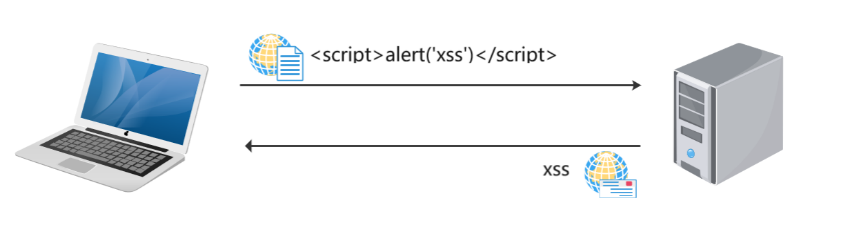
\includegraphics[width=3in]{figures/xss.png}
  \caption{Cross-Site Scripting (XSS)}
  \label{fig:xss}
  \end{figure}

XSS vulnerabilities typically arise due to the lack of input validation and output encoding when displaying user-generated content. It often caused by unqualified JavaScript code.

\begin{lstlisting}[caption={JavaScript Cross-Site Scripting (XSS)},label={lst:jsxss},language=HTML,breaklines=true]
var name = document.getElementById('name').value;
document.write("Welcome, " + name);
\end{lstlisting}

In this JavaScript example shown in \ref{lst:jsxss}, if the name value is not sanitized or encoded before being displayed using \verb|document.write()|, an attacker can inject JavaScript code as the value of name, leading to the execution of the injected script in the victim's browser.

\subsection{Server-Side Request Forgery (SSRF)}
Server-Side Request Forgery is a vulnerability where an attacker can manipulate a server's behavior by tricking it into making unintended or unauthorized requests to internal or external resources. This can lead to unauthorized access to sensitive information, port scanning, or even remote code execution. SSRF vulnerabilities typically occur when user-controlled input is used to construct URLs or make network requests without proper validation and access control.

\begin{lstlisting}[caption={Java Server-Side Request Forgery (SSRF)},label={lst:javassrf},language=JAVA,breaklines=true]
URL url = new URL(request.getParameter("url"));
HttpURLConnection connection = (HttpURLConnection) url.openConnection();
\end{lstlisting}

In the above Java code snippet in \ref{lst:javassrf}, if the user-provided url parameter is not properly validated or restricted, an attacker can supply a malicious URL that points to internal network resources, leading to SSRF.

\subsection{Remote Code Execution (RCE)}
Remote Code Execution is a severe vulnerability where an attacker can execute arbitrary code on a target system, potentially gaining full control over it. RCE vulnerabilities typically arise due to insecure coding practices, such as using user input directly in functions or commands without proper validation or sanitization. Attackers can exploit these vulnerabilities to run arbitrary commands, upload malicious files, or execute arbitrary code on the server.

\begin{lstlisting}[caption={PHP Remote Code Execution (RCE)},label={lst:phprce},language=PHP,breaklines=true]
$command = $_GET['command'];
exec($command);
\end{lstlisting}

In this PHP example in \ref{lst:phprce}, if the \verb|$_GET['command']| parameter is not properly validated or sanitized, an attacker can inject malicious commands, which will be executed by the exec() function, leading to arbitrary code execution on the server.

\subsection{URL Redirection}
URL Redirection vulnerabilities occur when untrusted user input is used to redirect users to unintended or malicious websites. Attackers can abuse this vulnerability to conduct phishing attacks, redirect users to malware distribution sites, or trick them into visiting unauthorized pages. This vulnerability arises when user-controlled input is directly used to construct redirect URLs without proper validation and sanitization.

\begin{lstlisting}[caption={Java URL Redirection},label={lst:javaurldr},language=JAVA,breaklines=true]
String redirectUrl = request.getParameter("redirect");
response.sendRedirect(redirectUrl);
\end{lstlisting}

In the above Java code in \ref{lst:javaurldr}, if the redirect parameter is not properly validated or restricted, an attacker can supply a malicious URL as the value, leading to unauthorized redirection of users to potentially harmful websites.

\subsection{Variable Overwriting}
Variable Overwriting vulnerabilities occur when the value of a variable can be controlled by an attacker, resulting in unexpected behavior or security issues in the code. This can happen due to insecure coding practices, such as allowing user input to directly modify critical variables without proper validation or sanitization, leading to unintended consequences or security breaches.

\begin{lstlisting}[caption={JavaScript Variable Overwriting},label={lst:jsvo},language=HTML,breaklines=true]
var isAdmin = false;
// Attacker-controlled input
isAdmin = true;
\end{lstlisting}

In this JavaScript example in \ref{lst:jsvo}, if the value of \verb|isAdmin| is influenced by user input without proper validation or access control, an attacker can overwrite the value of \verb|isAdmin| to true, potentially granting unauthorized administrative privileges.

\subsection{DNS poisoning}
DNS poisoning is a malicious attack aimed at disrupting the normal operation of the Domain Name System (DNS), which translates domain names to IP addresses. The principle behind DNS poisoning involves the manipulation of DNS responses to provide users with incorrect IP address or domain name mappings.
DNS poisoning can be categorized into two common attack methods: DNS cache poisoning and DNS hijacking.

\subsubsection{DNS cache poisoning}
In DNS cache poisoning, the attacker attempts to deceive recursive DNS servers into storing malicious DNS responses in their cache, which will be served to other users in subsequent queries, providing them with incorrect resolution results. The attacker sends DNS responses containing false IP address and domain name mappings, which may be mistaken as legitimate responses by recursive DNS servers and stored in their cache. When other users query the same domain, the recursive DNS server returns the cached incorrect response, redirecting the users to the wrong destination.

\subsubsection{DNS hijacking}
In DNS hijacking, the attacker attempts to intercept users' DNS requests and provide malicious DNS responses. The attacker may implement DNS hijacking through various means, such as setting up malicious DNS servers in infected routers or local networks or modifying DNS settings on users' devices through malicious software. When a user sends a DNS request, the attacker's malicious DNS server returns false IP address and domain name mappings, redirecting the user to a malicious website or server controlled by the attacker.

\subsection{Separation of front and back ends}
Front-end and back-end separation is a modern web development architecture, as shown in Fig.\ref{fig:Separation}, and design pattern that separates the front-end interface of the web page from the back-end server application logic, enhancing the maintainability of the application. Since front-end and back-end are independent, we can choose the technology stack that best suits our respective needs. For example, the front-end can use React, Vue.js or Angular, while the back-end can use Node.js, Python's Flask or Django, Ruby on Rails, etc. This separation improves development efficiency because development teams can independently update and extend different parts of the application without interfering with each other.

\begin{figure}[h]
  \centering
  
\includegraphics[width=2.5in]{figures/Preliminaries1.png}
  \caption{Separation of Front and Back ends}
  \label{fig:Separation}
  \end{figure}

\subsection{React for Front-End Development }
React is an open source JavaScript library widely used for building user interfaces. It allows developers to build applications using a componentized approach, meaning that each part of the user interface is encapsulated into independent, reusable components. React's responsive design principles ensure that the user interface can quickly respond to data changes. Fetch API is used for network requests in React applications. In this project, Fetch is used to communicate with the backend service to retrieve and send data.

\subsection{Ant Design of React}
Antd is a React UI library that follows the Ant Design specification and contains a set of high-quality components and demos for building rich interactive user interfaces.

\subsection{Cross-origin resource sharing}
Cross-origin resource sharing (CORS) is a security mechanism that allows or restricts resources on a web page (such as fonts, JavaScript, etc.) to be accessed by another domain name with a different origin. In the integration of React and Flask, CORS is an important consideration because the frontend and backend are usually deployed on different domains. Corresponding CORS strategies are used in this project to ensure safe and effective front-end and back-end communication.

\subsection{Postman}
Postman is an ideal tool for building and testing APIs. It supports all common HTTP request types, such as GET, POST, PUT, DELETE, etc. It allows users to easily add request parameters, header information, authentication data, etc. Postman provides a user-friendly interface that allows developers to easily send requests to the server and view the responses. By viewing the response data and status codes of the API, developers can quickly locate the problem.

\subsection{Flask for Back-End Development}
Flask is a lightweight web application framework written in Python. It is designed to be easily extensible and provides the necessary tools and features to build reliable web applications. In this project, Flask serves as the back-end framework to handle client requests and interact with the database.

\subsection{Database storage}
This project uses a database to store application data, which may include user information, transaction data, etc. In addition, the system supports file upload functionality, which is crucial for processing user-submitted code files. Flask provides integration with databases and the ability to handle file uploads.

\subsection{Nginx}
Nginx is a high-performance HTTP and reverse proxy server, which can also be used as a mail proxy server. In this project, Nginx is used as the web server, responsible for handling HTTP requests and forwarding them to the Flask application. The use of Nginx improves the reliability and load balancing capabilities of the application.

\subsection{Docker}
Docker is a popular open source containerization platform that allows developers to easily create, deploy, and run applications. By using Docker, developers can package applications and their dependencies into a portable container that can run on any Docker-enabled machine, ensuring application consistency across different environments.

\subsection{Kubernetes}
Kubernetes, also known as K8s, is an open-source container orchestration platform designed to automate the deployment, scaling, and management of containerized applications.  Kubernetes groups containers into logical units called pods, facilitating seamless management and discovery. Its core features include automated scaling, pod orchestration, services for networking, replication controllers, and deployments for ensuring application stability. With a master-node architecture, extensibility through Custom Resource Definitions (CRDs), and a vibrant community, Kubernetes has emerged as the industry standard, streamlining the complexities of containerized application deployment and management.


\section{Solution}
\noindent This section will introduce the structure of static code detection, as shown in Fig.\ref{fig:detectengine}. First, let's go over the functionality of each part:
\begin{itemize}
  \item File: This part holds the content of the file, along with related properties like the coding language and encoding format
  \item File Processing: Used to read the properties of the file, perform simple handling of the file, and check for read/write file errors
  \item Processing Unit: The central processing unit, responsible for invoking other modules when data is input
  \item Rules: Used to store detection rules, including rule description, matching rules, and error detection information, etc.
  \item Phraser: A semantic analyzer, which is used to analyze semantical errors in the code, build syntax trees, remove comments, etc.
  \item Detector: Detects errors in the code based on the rules
  \item Error Info: Stores error information detected in the code
  \item Output Module: Handles error information and generates corresponding XML/CSV files
\end{itemize}

\begin{figure}[h]
  \centering
  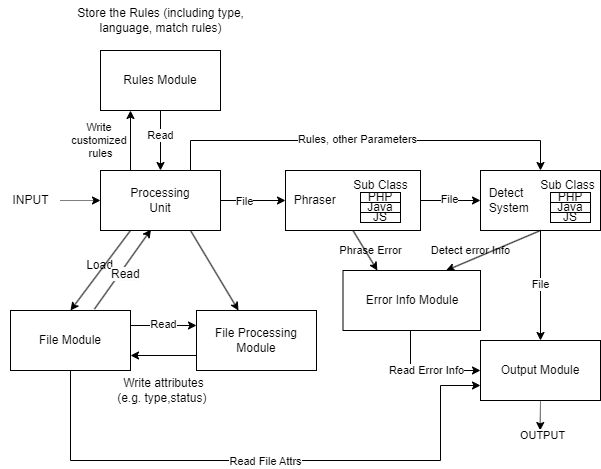
\includegraphics[width=3.3in]{figures/detectengine.png}
  \caption{Detect Engine}
  \label{fig:detectengine}
  \end{figure}

The design logic of this part has been mentioned in Sprint3 in \ref{sec:sprint3}, where we modularized the program and used abstract classes to comply with OCP (Open-Closed Principle) and LSP (Liskov Substitution Principle). When there is an input, the processing unit is responsible for invoking other modules, it will first let the file processing unit load the file and write the relevant File class, meanwhile, the processing unit will also read and write custom rules. After system initialization, it would input the corresponding files, rules, and other parameters into the semantic parser and detector, respectively. The detection information generated by the phraser and detector would be stored in a separate class, using a dedicated rule-error pair data structure. Finally, the output unit will read the class containing the detection information and output the corresponding documents based on this.

Compared to the original structure, this one encapsulates various parts (like rules, detection information) into corresponding classes. This not only hides the interfaces but also uses a relatively simple structure to protect the various modules and employs relatively simple interfaces to connect them. At the same time, the phraser and detector are handled as abstract classes, facilitating the extension of new detection languages in the future, thereby enhancing system scalability and reducing code duplication.

\subsection{Cross-Origin Resource Sharing}
Solving cross-domain problems is an important challenge in implementing a front-end and back-end separation architecture. Cross-Origin Resource Sharing (CORS) issues occur when a web page attempts to request resources from different sources (domain names, protocols, or ports). These requests may be rejected due to the browser's same-origin policy restrictions. Here are our ways to resolve cross-domain issues:

\subsubsection{Use CORS Headers}
The most common approach is to implement CORS on the server side. This can be achieved by adding specific CORS headers to the HTTP response. These headers tell the browser to allow web pages from different origins to access the resource. Allowing all sources can lead to security vulnerabilities, so we limit only specific, trusted sources.

\subsubsection{Reverse Proxy Server by Nginx}
Using a reverse proxy server between the front-end and back-end can effectively solve cross-domain issues, as shown in \ref{lst:nginxconf}. The proxy server receives the request sent by the front end and forwards the request to the actual backend server.

\begin{lstlisting}[caption={Nginx Configuration},label={lst:nginxconf},language=bash,breaklines=true]
server {
    listen 5003;
    server_name _;
    location / {
	if ($request_method = 'OPTIONS') {
            add_header 'Access-Control-Allow-Origin' 'http://127.0.0.1:3000';
            add_header 'Access-Control-Allow-Methods' 'GET, POST, OPTIONS';
            add_header 'Access-Control-Allow-Headers' 'Content-Type, Authorization';
            add_header 'Access-Control-Allow-Credentials' 'true';
            add_header 'Content-Length' 0;
            add_header 'Content-Type' 'text/plain; charset=utf-8';
            return 204;
        }

        if ($request_method = 'POST') {
            add_header 'Access-Control-Allow-Origin' 'http://127.0.0.1:3000';
            add_header 'Access-Control-Allow-Methods' 'GET, POST, OPTIONS';
            add_header 'Access-Control-Allow-Headers' 'Content-Type, Authorization';
            add_header 'Access-Control-Allow-Credentials' 'true';
        }

        if ($request_method = 'GET') {
            add_header 'Access-Control-Allow-Origin' 'http://127.0.0.1:3000';
            add_header 'Access-Control-Allow-Methods' 'GET, POST, OPTIONS';
            add_header 'Access-Control-Allow-Headers' 'Content-Type, Authorization';
            add_header 'Access-Control-Allow-Credentials' 'true';
        }
        proxy_pass http://127.0.0.1:5000/;
        proxy_set_header X-Forwarded-For $proxy_add_x_forwarded_for;
        proxy_set_header X-Forwarded-Proto $scheme;
        proxy_set_header X-Forwarded-Host $host;
        proxy_set_header X-Forwarded-Prefix /;
    }
}
\end{lstlisting}

\subsection{Interface adjustment and troubleshooting, communication between front-end and back-end}
During the software engineering process, effective communication between front-end and back-end teams is critical to successfully tuning interfaces. Postman is a powerful tool that can play a key role in this process. The following are the steps to use Postman to communicate with the back-end interface, adjust the interface, and troubleshoot based on the software engineering process:
\subsubsection{Define and understand interface specifications}
\begin{itemize}
  \item Requirements analysis: In the early stages of development, our front-end and back-end teams jointly reviewed functional requirements and clarify the purpose and expected behavior of the interface.
  \item Interface documentation: Backend teams created detailed interface documentation, including endpoint URLs, request methods (GET, POST, etc.), request parameters, expected response formats, and status codes, as shown in Fig.\ref{fig:interfacespec}.
  \item Review and feedback: Our front-end team reviewed these documents and ask questions or request changes.
\end{itemize}

\begin{figure}[h]
  \centering
  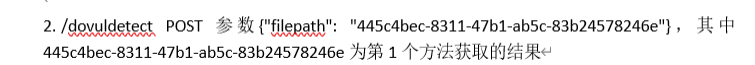
\includegraphics[width=3.2in]{figures/solution-interspec.png}
  \caption{Interface documentation}
  \label{fig:interfacespec}
  \end{figure}

\subsubsection{Use Postman(Fig.\ref{fig:postman}) for interface testing}
\begin{itemize}
  \item Write a request: According to the interface document, set the URL, method, header, parameters, etc. of the request.
  \item Send a request: Execute the request and observe the response. Check whether the response status code, data structure and data content are as expected.
\end{itemize}

\begin{figure}[!t]
  \centering
  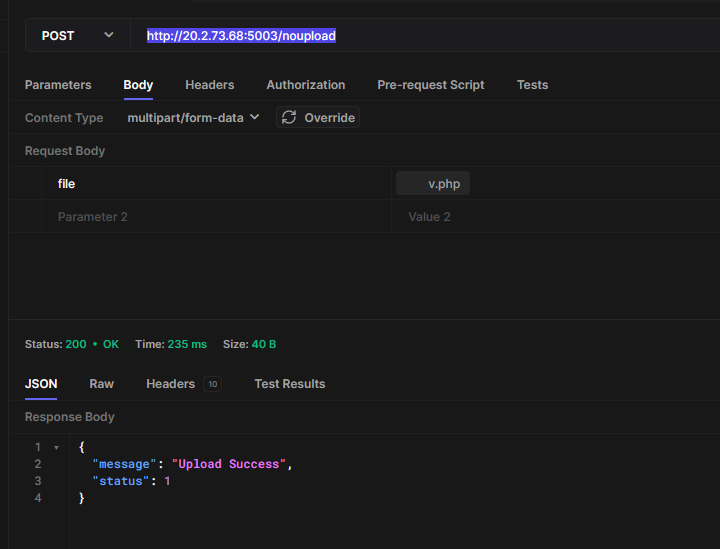
\includegraphics[width=3in]{figures/solution-postman.png}
  \caption{Postman for interface testing}
  \label{fig:postman}
  \end{figure}

\subsubsection{Interface debugging and troubleshooting}
\begin{itemize}
  \item Record and share results: Use Postman's to record and share test results with your backend team, especially when issues were discovered.
  \item Error identification: For error responses, analyze the error message or status code in the response body to determine the nature of the error.
\end{itemize}
\subsubsection{Communication and collaboration}
\begin{itemize}
  \item Feedback and modifications: Feed back the problems discovered during testing to the backend team and discuss how to modify the interface to meet needs.
  \item Update documentation: Once the interface changes, make sure to update the interface documentation to keep the documentation up-to-date.
  \item Iterative testing: Repeat testing of the modified interface to ensure that all issues have been resolved.
\end{itemize}

\begin{figure*} 
  \centering
\subfloat[\label{1a}]{%
     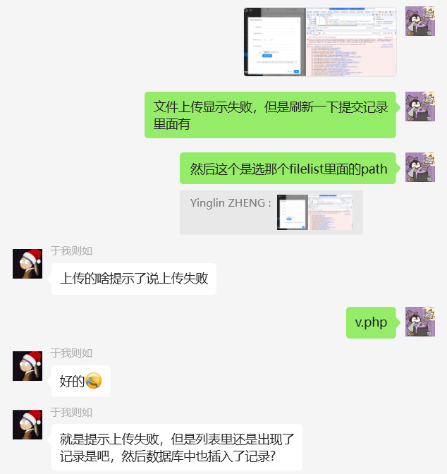
\includegraphics[height=2in,width=0.3\textwidth]{figures/collaboration1.png}}
  \hfill
\subfloat[\label{1b}]{%
      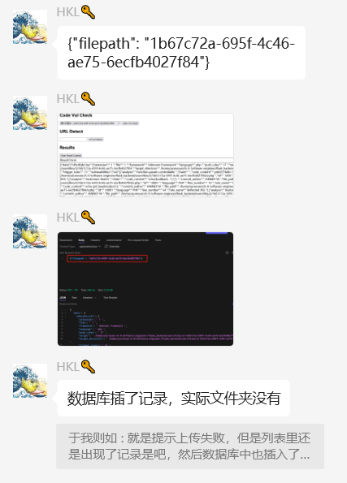
\includegraphics[height=2in,width=0.3\textwidth]{figures/collaboration2.png}}
  \hfill
\subfloat[\label{1c}]{%
      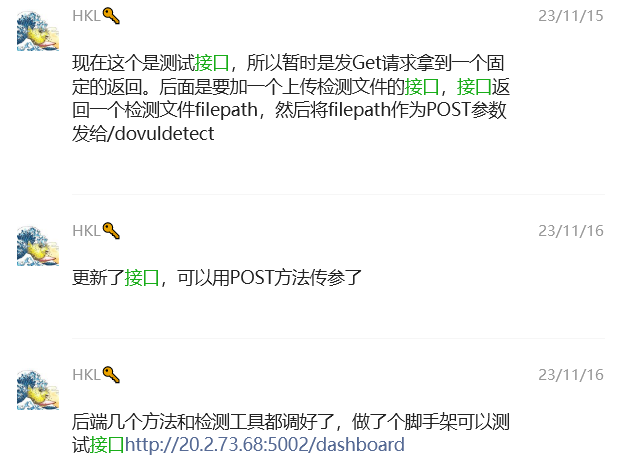
\includegraphics[height=2in,width=0.3\textwidth]{figures/collaboration3.png}}
  \hfill
  \\
\subfloat[\label{1d}]{%
      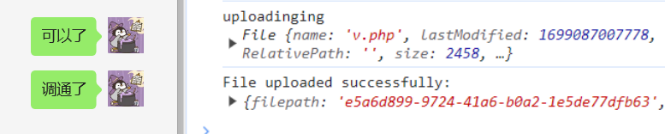
\includegraphics[height=0.8in,width=0.5\textwidth]{figures/collaboration4.png}}
\caption{(a), (b) Feed back the problems discovered during testing to the backend team and discuss how to modify the interface to meet needs.(c) Once the interface changes, make sure to update the interface documentation to keep the documentation up-to-date,(d) Iterative testing: Repeat testing of the modified interface to ensure that all issues have been resolved.}
\label{fig:collaboration} 
\end{figure*}


\subsection{Collaboration between different front-end developers}
In the software engineering process, using Git for version control and branch management is a common practice, especially in projects where multiple people collaborate. The following is the branch strategy of our front-end development team based on Git.
\subsubsection{Create a front-end branch}
Create a development branch (front-end) from the main branch. This branch contains all the latest front-end development work.
\subsubsection{Separate feature branches from the development branch}
Each developer creates his or her own branch (Yinglin-ZHENG, Xi-CHEN, etc.) from the development branch to develop assigned functional tasks or fix bugs, which ensures that development work is independent of each other and reduces conflicts.
\subsubsection{Add Readable commits and Request Review for Merge}
Developers committed their code with readable information and requested review and test from each other's, then wait for other coders to make comment, if the function is completed correctly, it can be merged into front-end branch. If there are something conflict when merge, we made a discussion between the code writers.

\subsection{Deal With JSON Response in front-end}
\subsubsection{Data interaction and analysis}
\begin{itemize}
  \item Receive JSON data: The front end receives a JSON formatted response from the back end. This is achieved by using the Fetch API and processing the response, as shown in Fig.\ref{fig:datainteana1a}.
  \item Parse JSON: The front-end application parses JSON data and converts it into JavaScript objects for further processing and display, as shown in Fig.\ref{fig:datainteana1b}.
\end{itemize}

\begin{figure} 
  \centering
\subfloat[Receive JSON data\label{fig:datainteana1a}]{%
     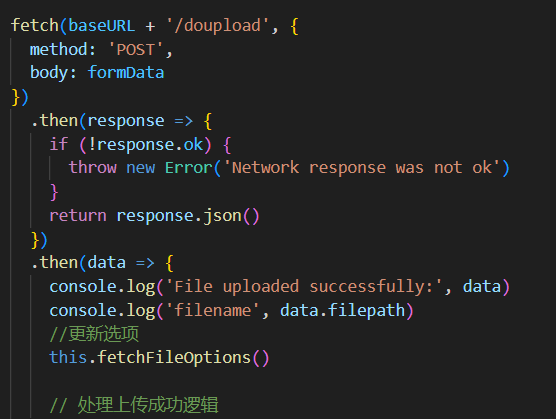
\includegraphics[height=2in,width=0.45\linewidth]{figures/json1.png}}
  \hfill
\subfloat[Parse JSON\label{fig:datainteana1b}]{%
      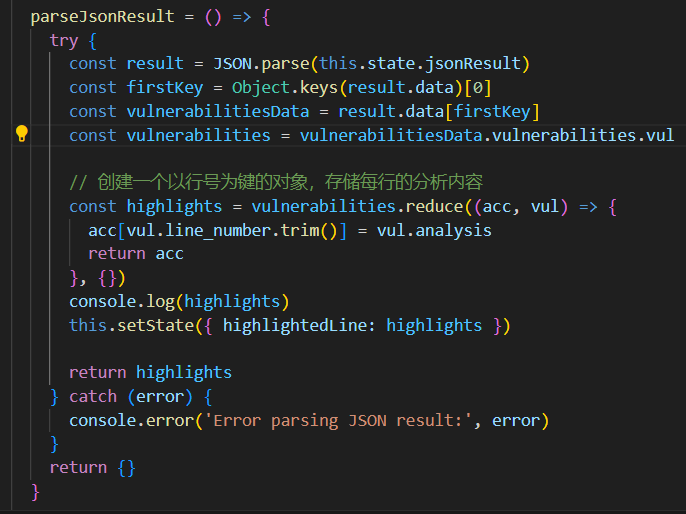
\includegraphics[height=2in,width=0.45\linewidth]{figures/json2.png}}
\caption{Data interaction and analysis}
\label{fig:datainteana} 
\end{figure}

\subsubsection{Front-end interface design}

\begin{itemize}
  \item Display code: Use appropriate HTML elements such as \verb|<pre>| and \verb|<code>| tags to display code, as shown in Fig.\ref{fig:displaycode}.
  \item Code highlighting: Use front-end libraries highlight.js, to implement code highlighting, as shown in Fig.\ref{fig:highlightcode}. 
\end{itemize}

\begin{figure}[h]
  \centering
  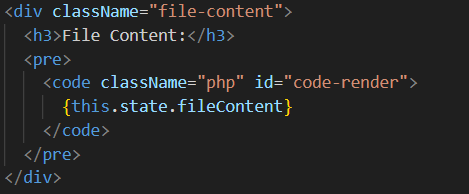
\includegraphics[width=2in]{figures/displaycode.png}
  \caption{Display code}
  \label{fig:displaycode}
  \end{figure}

\begin{figure}[h]
  \centering
  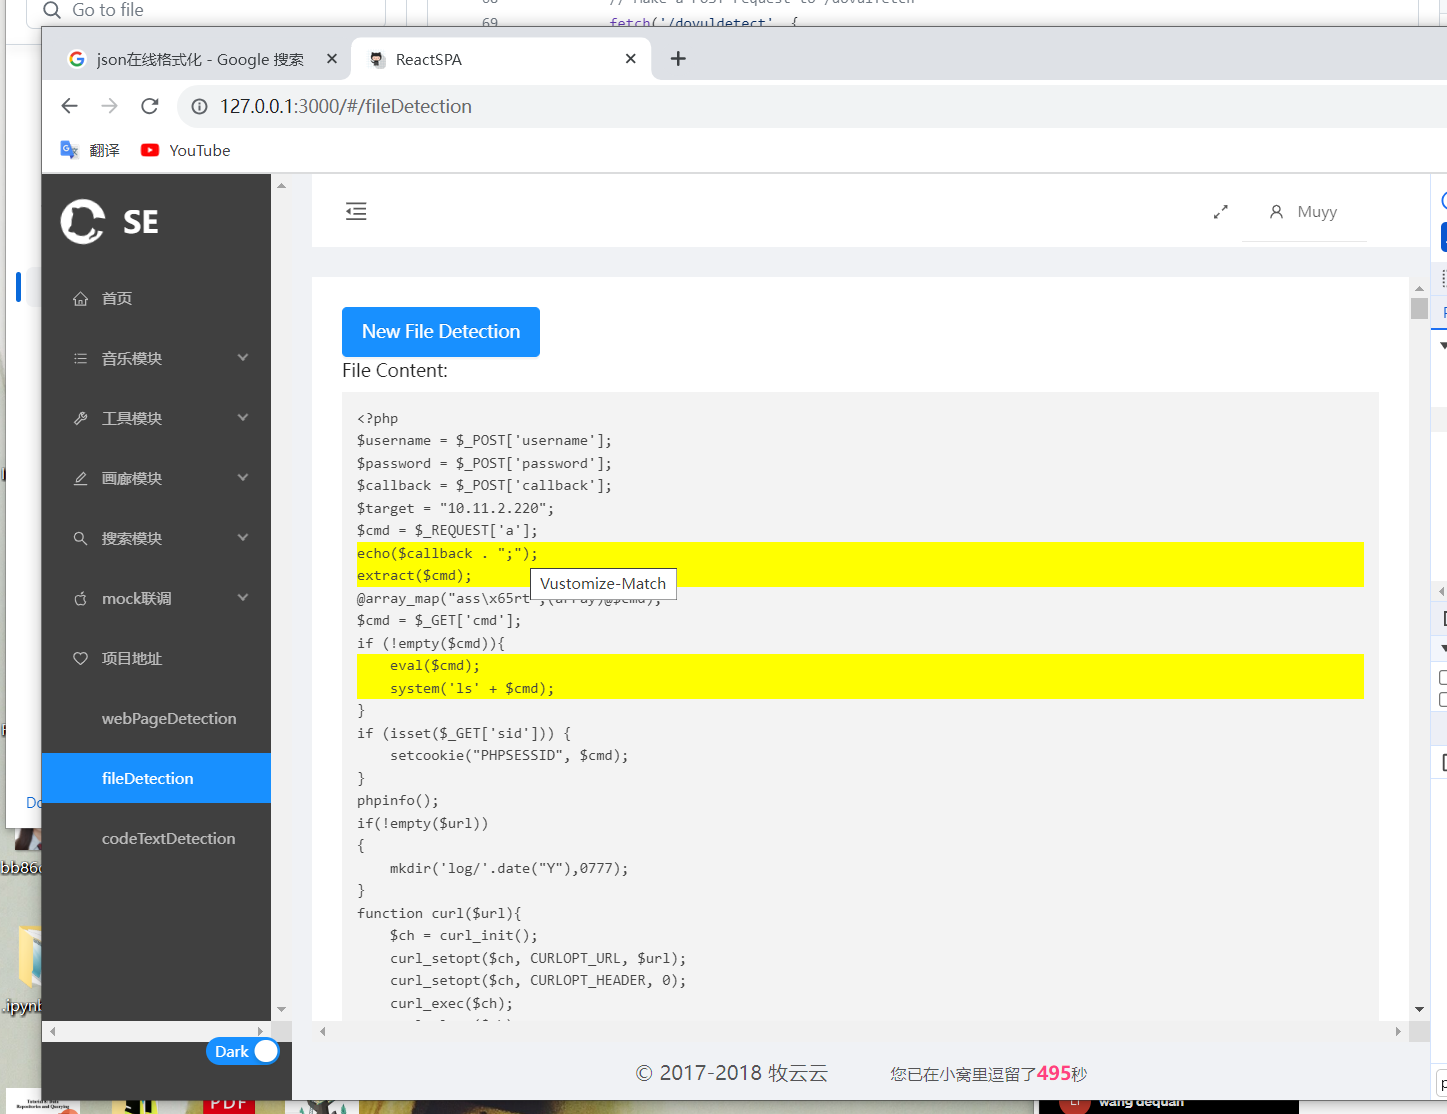
\includegraphics[width=3in]{figures/highlightcode.png}
  \caption{Code highlighting}
  \label{fig:highlightcode}
  \end{figure}

\subsubsection{Implementation of interactive functions}
\begin{itemize}
  \item Hover tip implementation: When the mouse hovers over a specific code segment, a tooltip is displayed to display the vulnerability analysis of the code segment.
  \item Correlate vulnerability data: Store vulnerability analysis metadata (e.g. using data-attributes) in each highlighted section of code for retrieval and display on hover.
\end{itemize}


\subsection{Reusable component implementation}
\subsubsection{Requirement analysis}
\begin{itemize}
  \item Functional requirements: Determine the functions that the component needs to support, such as user input, confirm/cancel buttons, close icons, etc.
  \item User interface requirements: Define the appearance of the pop-up window, including size, etc.
\end{itemize}

\subsubsection{Design}
\begin{itemize}
  \item Architecture design: designing component as an independent reusable component.
  \item Interface design: Create interface prototypes or design drawings of pop-up components.
  \item Interaction design: Plan how users interact with pop-up windows, such as handling click events.
\end{itemize}

\subsubsection{Implementation}
\begin{itemize}
  \item Create React components using antd UI style
  \item State management: Manage the display/hidden state of the componets ( such as pop-up window)
\end{itemize}

\subsubsection{Test}
\begin{itemize}
  \item Ensure that the appearance and interaction of the pop-up window meet the design requirements.
  \item Collect feedback on popup components from users or stakeholders
\end{itemize}

\subsection{Using modern code review to address code execution issues}
After completing and testing the algorithmic code for the safety detection of the web portion, Author Wang Xiaoxuan uploads this code to GitHub and notifies two reviewers, Kong Wenkai and Huang Kunlun, via email to review the code for functionality, readability, and robustness. Eventually, reviewer Kong Wenkai discovers a code vulnerability that prevents the code from running on the server and notifies author wangxiaoxuan. After fixing the bug, author wangxiaoxuan re-uploads the code.

\begin{figure}[h]
  \centering
\subfloat[First Code Submission Record\label{fig:mcrsub}]{%
     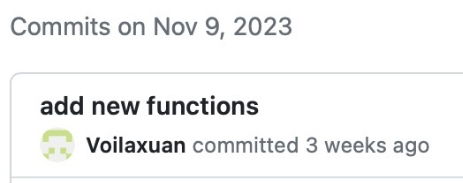
\includegraphics[width=0.9\linewidth]{figures/mcrsub.png}}
  \hfill
\subfloat[Reviewer submitted comments on the bugs found\label{fig:mcrinter}]{%
      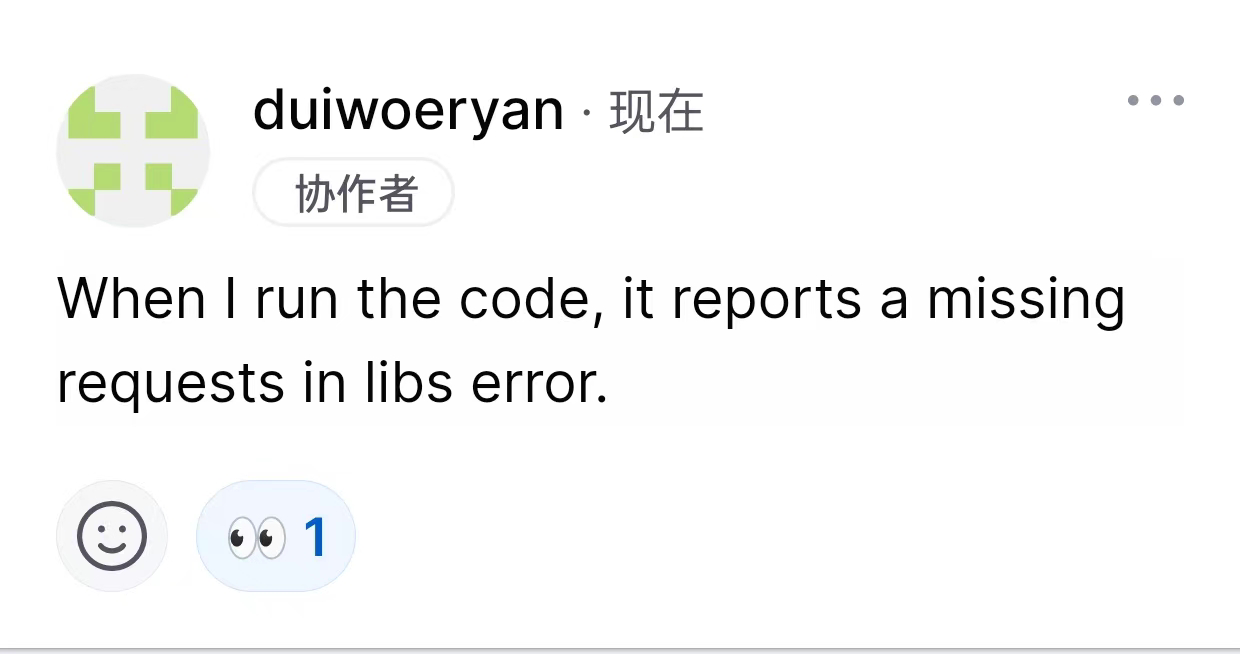
\includegraphics[width=0.9\linewidth]{figures/mcrinter.png}}
  \hfill
\subfloat[Fix bug\label{fig:mcrfixbug}]{%
      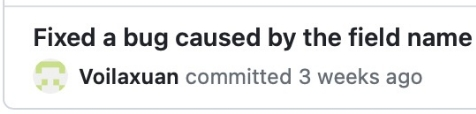
\includegraphics[width=0.9\linewidth]{figures/mcrfixbug.png}}
\caption{Modern Code Review}
\label{fig:mcr} 
\end{figure}

\subsection{Multi-Platform}

To maximize accessibility, our tool is designed for deployment in diverse scenarios, with a focus on both user-friendly web access and a simplified GUI for desktop users. This approach aligns with the principles of usability and adaptability emphasized in software engineering.

\subsubsection{B/S-Based Application}

Our primary deployment targets a Browser/Server (B/S) architecture, providing users with a seamless and user-friendly experience. This platform-independent approach ensures that developers can easily access and utilize our tool without the need for specific operating systems or installations. This aligns with software engineering emphasis on web-based technologies and their relevance in modern software development.

\subsubsection{Desktop GUI}

Recognizing the diversity in developer preferences and environments, we also provide a straightforward Graphical User Interface (GUI) for desktop users. This option ensures that our tool caters to developers who may prefer a local installation or work within specific desktop environments. This versatility resonates with the adaptability concepts covered in software engineering.
\begin{figure}[h]
\centering
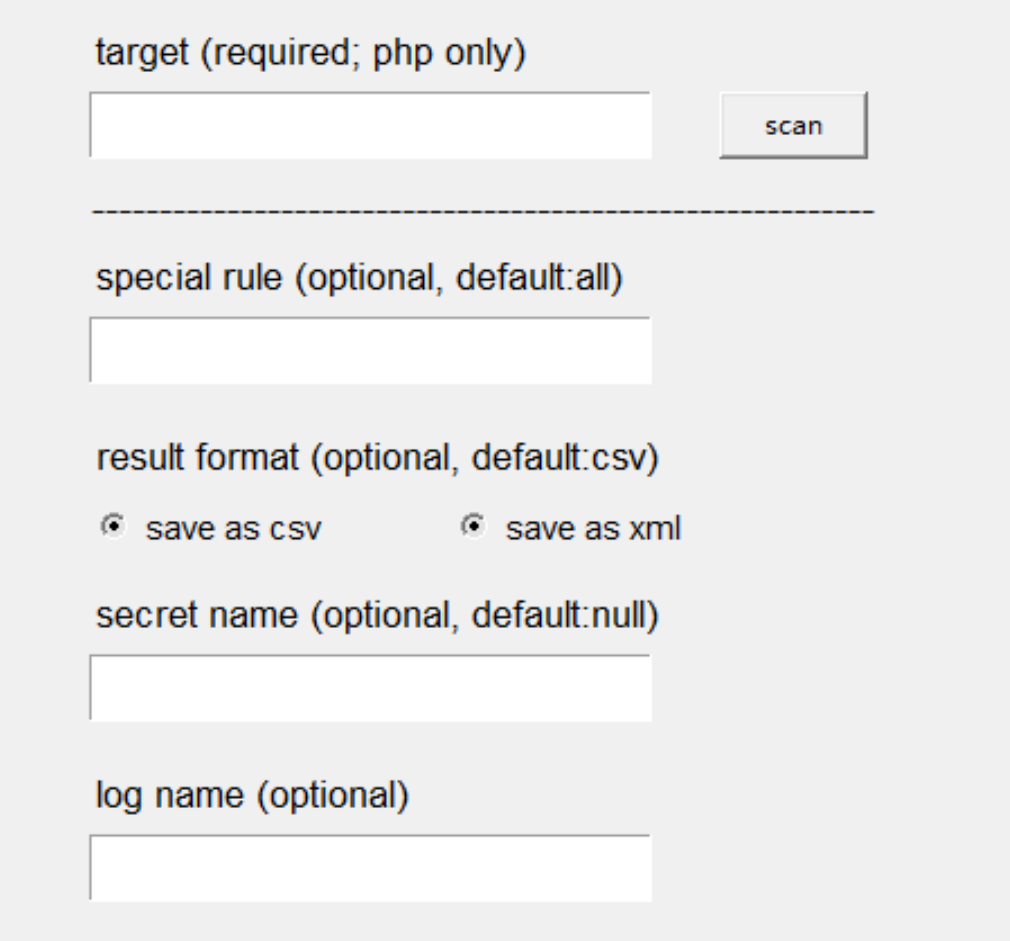
\includegraphics[width=2in]{figures/guimulti.png}
\caption{Desktop GUI}
\label{fig:guimul}
\end{figure}


\subsection{DevOps Integration}
\label{sol:devops}

In keeping with contemporary software engineering practices, our tool is deployed using robust DevOps practices, aligning with the DevOps principles covered in software engineering.

\subsubsection{Cloud Deployment on Microsoft Azure}

We leverage Microsoft Azure for cloud deployment, offering scalability, reliability, and a range of services that enhance the overall performance of our tool. This choice aligns with software engineering's coverage of cloud computing and its role in modern software development.

\subsubsection{Containerization with Docker}

To enhance portability and consistency across different environments, we utilize Docker for containerization. This allows our tool and its dependencies to be packaged together, ensuring that it runs consistently on various platforms. This aligns with software engineering's coverage of containerization and its impact on software deployment.

\begin{algorithm}[hbt!]
    \caption{Scalability Model}\label{alg:Scalabilitymodel}
    \begin{algorithmic}
    
    \Require $Deployment\ Definition$
  
    \State Initialization($Deployment\ Definition$) 

    \Repeat
        \State Monitoring($sys\_Status$)
        \State $New\ Definition$ $\gets$ Replica\_Calculation($sys\_Status$)
        \State Initialization($New\ Definition$) 
    \Until{$Done$}
    
    \end{algorithmic}
  \end{algorithm}

\subsubsection{Kubernetes for Scalability}

Ensuring our tool's robustness and scalability, we employ Kubernetes for container orchestration in algorithm \ref{alg:Scalabilitymodel}. This choice aligns with software engineering's exploration of scalable architectures and their significance in handling diverse workloads efficiently.
\begin{figure}[h]
\centering

\includegraphics[width=1.6in]{figures/k8slogo.png}
\caption{Employing DevOps Techniques.}
\label{fig:k8slogo}
\end{figure}


\section{Software Process}
\noindent The Software Process section documents the team's activities throughout the project, highlighting the achievements of each sprint. Each sprint is elaborated on in two pages, capturing the essence of the tasks undertaken, challenges faced, and milestones achieved. Additionally, the section includes a burndown chart, offering a visual representation of project progress throughout its duration.

\subsection{The 1st Sprint}

This sprint focused on defining the scope and objectives, selecting the programing framework, and designing the user interface. The goal was to lay the foundation for the development of a comprehensive software.

\subsubsection{Defining the scope and objectives}

Defining the scope and objectives can be divided into the following two stages:

\textbf{Requirements gathering and analysis:}

Before determining the theme of this software development, the team members interviewed their university classmates and former colleagues on the question "As a programmer, what do you think are the pain points in development?" Through the collection and analysis of the interview content, we draw a conclusion: 

Generally, before a website is launched, the code and the developed website need to undergo security testing, and only after the test is passed can the version be launched.However, in all companies, code security and website security are two different tools, and some are even carried out in two separate departments, which means that this can greatly reduce the efficiency of programmers. Therefore, after discussion, our group unanimously agreed to develop a safety detection tool, which can realize synchronous scanning of web security vulnerabilities and code security vulnerabilities.

\textbf{Requirements validation and prioritization:}
This security scanning tool is divided into two parts: web security scanning and code security scanning. 

For web security scanning, the following requirements are identified and prioritized from high to low:
\begin{itemize}
  \item Home page probe IP: This is the fundamental functionality for a website scanning tool.
  \item SQL injection vulnerability detection: It enables the timely discovery and remediation of existing vulnerabilities to prevent attackers from exploiting SQL injection attacks to gain sensitive data or compromise the database, thereby enhancing system security and data protection capabilities.
  \item Common port detection: Conducting port detection helps in identifying open ports in the network system, promptly recognizing potential security risks and vulnerabilities, strengthening system security configurations and defense measures, and preventing unauthorized access and attacks.
  \item DNS spoofing detection: Detecting DNS pollution enables early discovery of malicious activities, preventing users from being redirected to malicious websites or falling victim to phishing attacks, thereby protecting user privacy and data security. It also improves network performance and reliability by ensuring accurate and reliable domain name resolution
  \item Web directory blasting:Web directory blasting can help identify hidden vulnerabilities, sensitive information, and misconfigurations on a website, enhancing access control and security measures to prevent potential exploitation and unauthorized access.
\end{itemize}
For the code security scanning part, we have selected three popular programming languages for detection: PHP, Java, and JavaScript.
By including PHP, Java, and JavaScript in the code security scanning, we can effectively identify and address security vulnerabilities, coding errors, and potential weaknesses specific to these languages. This comprehensive approach helps ensure the overall security and integrity of the codebase across different programming languages.

\textbf{Non-functional requirements:}

\textbf{Security:}
\begin{itemize}
  \item Implement a login interface where users need to provide a username and password to access the system's functionality. 
  This requirement helps protect sensitive information and ensures that only authorized personnel can access the system. It allows for tracking user activity and recording important events. Audit tracking is valuable for security and compliance, enabling administrators to monitor user behavior, detect any unauthorized activities, and hold users accountable for their actions in the system.

  \item Encrypt the password field of the database users. 
  Encrypting the user's password field enhances data security, protects sensitive user information, and prevents malicious use of passwords. Encryption helps safeguard user privacy and prevents unauthorized individuals from directly viewing the user's original password. Encrypting aligns with industry and regulatory compliance requirements, ensuring compliance with data protection and privacy regulations. In the event of a data breach, encrypted passwords reduce the risk of unauthorized access since decrypting the passwords requires a decryption key. Implementing password encryption demonstrates a commitment to data security, enhancing user trust and confidence in the system's ability to protect sensitive information.

\end{itemize}

\textbf{Maintainability:}
Divide the software development into three modules: frontend, backend, and algorithm. 
Firstly, modular design allows for clear separation and understanding of responsibilities among the modules, reducing code complexity. Secondly, independent development and testing of different modules facilitate parallel work and rapid iterations, improving development efficiency. Additionally, modular structure enhances code reusability, enabling precise localization and adjustment when modifying or optimizing a specific module, minimizing the impact on the entire system.

\textbf{Testability:}
Encapsulate each functionality into an interface. 
Interfaces define the inputs and outputs of functionalities, making testing clear and controllable by validating different inputs and expected outputs. The presence of interfaces allows for testing functionalities in isolated testing environments, unaffected by other functionalities, enhancing repeatability and reliability. Furthermore, interfaces encourage modular and decoupled design, facilitating testing and early detection and resolution of issues. By conducting automated tests on interfaces, testing efficiency is improved, reducing the workload of manual testing and accelerating software delivery. Overall, presenting each functionality as an interface enhances the testability of the software system, reducing testing complexity, and improving accuracy and efficiency.

\subsubsection{Selecting the programing framework}
Different frameworks have been chosen for frontend, backend, and algorithm.

\textbf{Frontend:} During the initial design discussions, we considered both Vue and React frameworks for the frontend. After researching and practical experiments, we select React as frontend framework for the following reasons:

\begin{itemize}
  \item Flexibility and customizability: React provides a flexible API and hooks, allowing developers to customize the components according to the project's requirements. React also supports integration with other libraries and frameworks, giving developers the option to choose the tools that best suit their needs.
  \item Component-based development: React is a component-based framework that allows developers to break down the user interface into reusable components. This modular approach makes the code more manageable and maintainable. For a complex security scanning tool, this modular development approach offers flexibility and efficiency.
\end{itemize}

\textbf{Backend and Algorithm:} For the backend and algorithm frameworks, we considered Flask, Django, Tornado, and Cubes during the initial design discussions. We decided to go with the Flask framework for the following reasons:
\begin{itemize}
\item Compared to Django:
Flask is more lightweight and flexible compared to Django, which includes a large set of built-in components and functionalities. This makes Flask more suitable for small or medium-sized projects and projects that require a higher level of customization.
Flask provides fewer abstractions and constraints, allowing developers more freedom in choosing and integrating third-party libraries. It is also well-suited for building RESTful APIs and microservices.
\item Compared to Tornado:
Flask offers a more comprehensive ecosystem and a larger community support, making it easier to find the required plugins, tools, and documentation throughout the development process.
Tornado is primarily designed for high-performance asynchronous web applications, which excel in handling a large number of concurrent requests. However, for a general security scanning tool, asynchronous performance is not a primary requirement. Flask's synchronous approach is simpler and more developer-friendly.
\item Compared to Cubes:
Cubes is a framework focused on building analytical and reporting applications, with a strong emphasis on data visualization and analysis. In contrast, a security scanning tool primarily focuses on vulnerability scanning and code security. Therefore, Flask is more suitable for the development of the backend and algorithm components.
\end{itemize}

\subsubsection{Designing the user interface} Including the Interface between Backend and algorithm and Interface between Backend and Frontend

\textbf{Interface between Backend and algorithm}

The development team of the algorithm group will write each functionality as a method, and finally encapsulate the code security scanning functionality and web security scanning functionality into separate libraries, which will be called by the backend collectively.

\begin{figure}[h]
  \centering
  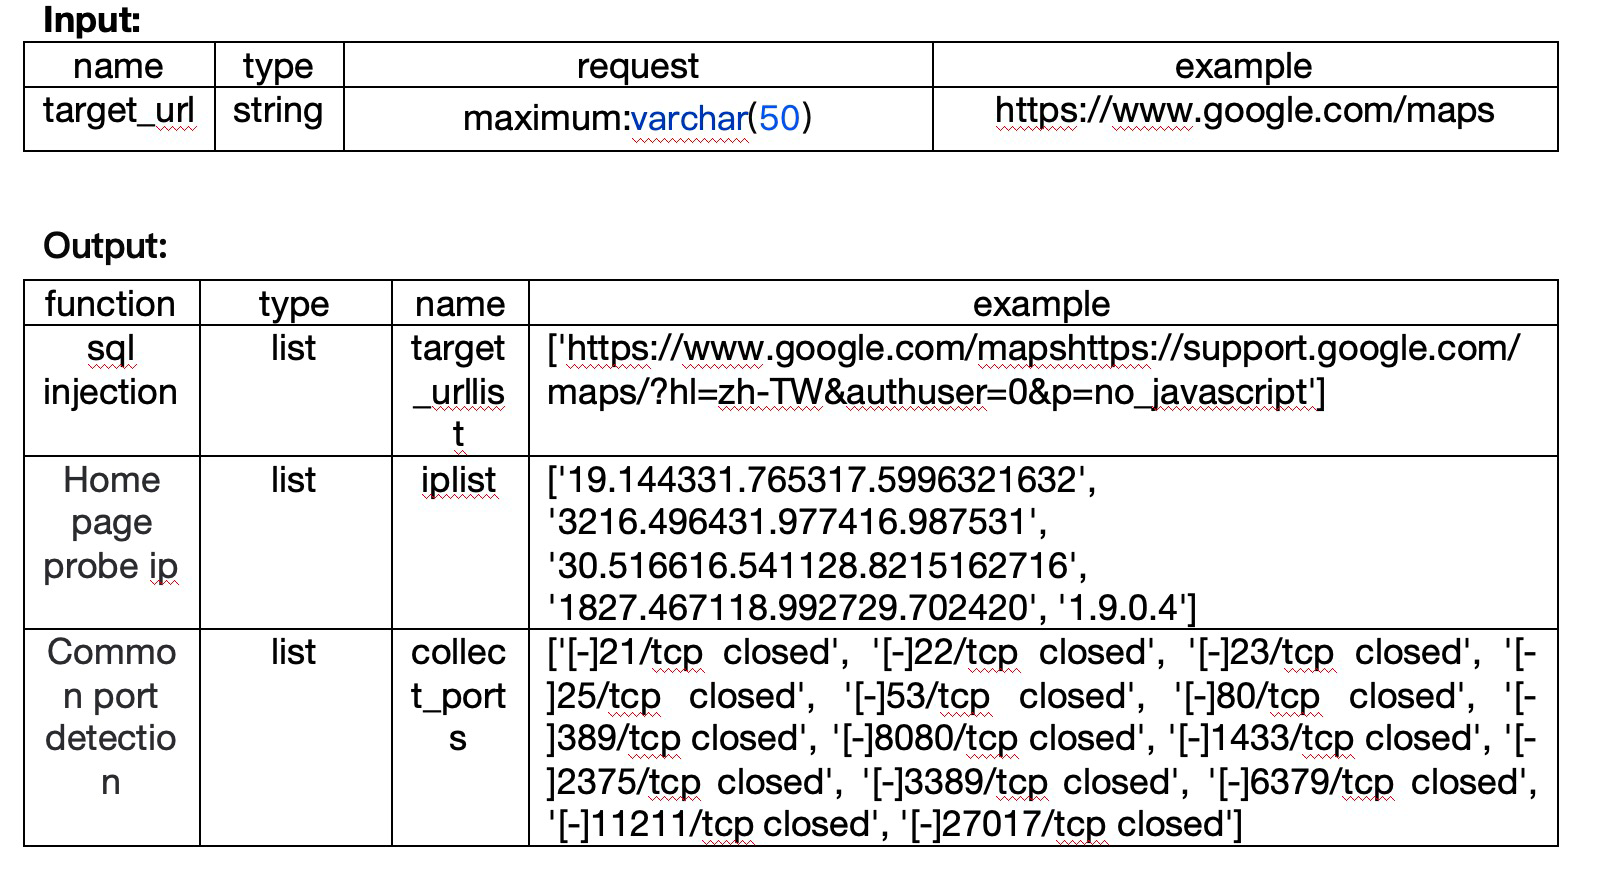
\includegraphics[width=3.4in]{figures/sprintapidoc1.png}
  \caption{Partial API Documentation}
  \label{fig:sprintapidoc1}
  \end{figure}

\textbf{Interface between Backend and Frontend}
The backend will deploy the code to the server at Microsoft Azure Cloud Server. The frontend will use the POST method to send requests. The API documentation is as follows shown in Fig.\ref{fig:sprintapidoc2}.
\begin{figure}[h]
  \centering
  \includegraphics[width=3.4in]{figures/sprintapidoc2.png}
  \caption{Partial API Documentation}
  \label{fig:sprintapidoc2}
  \end{figure}

\subsection{The 2nd Sprint}
The task of this sprint is to complete the development of front-end, back-end, and algorithm code, integrate and debug the front-end, back-end, and algorithm code, and continuously improve and optimize the functionality by debugging bugs. The goal is to create a software that can be delivered for basic use. In this sprint, the three tasks actually overlap with each other. The first task to start is the development of front-end, back-end, and algorithm code. Shortly after the development starts, code evaluation and bug testing are conducted to identify and resolve any potential bugs in the early stages of development and to find better coding methods. By simultaneously developing and testing during the development process, potential errors and defects can be detected early, which helps in timely problem fixing and avoids the escalation of issues or more serious consequences in later stages of development. At the same time, identifying and resolving issues early in the code development phase is more cost-effective and efficient than doing it later. If problems are discovered and addressed only in the later stages, the amount of work and cost required for fixing them may be greater.

\subsubsection{Front-end, Back-end, and Algorithm Development}
The development tasks of the code lasted almost the entire duration of sprint 2, from October 4, 2023, to October 24, 2023. The development of the code aimed to deliver a usable code within the sprint 2 cycle. We divided the code development into three parts, each assigned to different team members: front-end, back-end, and algorithm. By allocating resources appropriately, we were able to effectively expedite the project development process. 

\subsubsection{Front-end, Back-end, and Algorithm Development}
The development tasks of the code lasted almost the entire duration of sprint 2, from October 4, 2023, to October 24, 2023. The development of the code aimed to deliver a usable code within the sprint 2 cycle. We divided the code development into three parts, each assigned to different team members: front-end, back-end, and algorithm. By allocating resources appropriately, we were able to effectively expedite the project development process.

First and foremost is the crucial algorithm part. We created two sets of algorithm code for website security scanning and code security scanning, respectively. For website security scanning, the following requirements were determined and ranked from high to low: homepage IP detection, SQL injection vulnerability detection, common port detection, DNS spoofing detection, and web directory brute-forcing. As for code security scanning, the target requirement of this project is to support the detection of various vulnerabilities in code written in different languages. In this sprint, we have completed all the requirements for website security scanning, and for code security scanning, we have developed vulnerability scanning for JavaScript (JS), PHP, and Java, as shown in Table \ref{tab:vulscanft}. Due to time constraints, we couldn't include more vulnerability types for website and code scanning, which is a regret in this sprint.

% Please add the following required packages to your document preamble:
% \usepackage[table,xcdraw]{xcolor}
% Beamer presentation requires \usepackage{colortbl} instead of \usepackage[table,xcdraw]{xcolor}
\begin{table}[h]
    \centering
  \caption{Vulnerability Scanning Features}
  \label{tab:vulscanft}
  \begin{tabular}{|c|c|c|c|}
    \hline
    \multicolumn{1}{|l|}{}         & \multicolumn{1}{l|}{PHP} & \multicolumn{1}{l|}{JS} & \multicolumn{1}{l|}{java} \\ \hline
    XSS                            & \checkmark                        & \checkmark                       & \multicolumn{1}{l|}{}     \\ \hline
    SSRF                           & \checkmark                        &                         & \checkmark                         \\ \hline
    SQL injection                  & \checkmark                        & \checkmark                       &                           \\ \hline
    remote file include            & \checkmark                        & \checkmark                       &                           \\ \hline
    Xml injection                  & \checkmark                        &                         &                           \\ \hline
    Remote code execute            & \checkmark                        & \checkmark                       &                           \\ \hline
    LDAP injection                 & \checkmark                        &                         &                           \\ \hline
    Information Disclosure         & \checkmark                        &                         &                           \\ \hline
    URL Redirector Abuse           & \checkmark                        &                         &                           \\ \hline
    variable shadowing             & \checkmark                        &                         &                           \\ \hline
    unserialize vulerablity        & \checkmark                        & \checkmark                       & \checkmark                         \\ \hline
    CSRF                           &                          & \checkmark                       & \checkmark                         \\ \hline
    Server-Side Template Injection &                          & \checkmark                       &                           \\ \hline
    Command Injection              &                          & \checkmark                       &                           \\ \hline
    XXE                            &                          &                         & \checkmark                         \\ \hline
    File upload vulnerability      &                          &                         & \checkmark                         \\ \hline
    Remote command execute         &                          &                         & \checkmark                         \\ \hline
    \end{tabular}
  \end{table}


The most important task for the backend part is to provide business logic to the frontend based on algorithms and perform calculations based on frontend requests. Additionally, there are requirements for database management and security verification, such as interacting with the database for data storage, retrieval, and updates, as well as ensuring user login authentication. In this sprint, the backend completed the aforementioned tasks, but there were some non-functional requirements that were not met, such as inadequate support for high-frequency API calls in terms of performance. Due to development speed, we chose Python for backend development. Python is an interpreted language and may not be as efficient in terms of performance as compiled languages like Java with Spring Boot.

\textbf{Backend Development}
The most important task for the backend part is to provide business logic to the frontend based on algorithms and perform calculations based on frontend requests. Additionally, there are requirements for database management and security verification, such as interacting with the database for data storage, retrieval, and updates, as well as ensuring user login authentication. In this sprint, the backend completed the aforementioned tasks, but there were some non-functional requirements that were not met, such as inadequate support for high-frequency API calls in terms of performance. Due to development speed, we chose Python for backend development. Python is an interpreted language and may not be as efficient in terms of performance as compiled languages like Java with Spring Boot.

\textbf{Frontend Development}
In this sprint, the main functional requirements for frontend code development were: 
\begin{enumerate}[(i)]
  \item providing users with a webpage for website security scanning, and 
  \item providing users with a webpage for code security scanning. 
\end{enumerate}
The non-functional requirements included: 
\begin{enumerate}[(i)]
\item providing users with a visually appealing interface, 
\item offering a navigation bar for user convenience, and 
\item enabling users to write code directly on the webpage. 
\end{enumerate}
In terms of functional requirements, we fully completed them in this sprint by providing two different interfaces for website security scanning and code security scanning. All non-functional requirements, except for the ability to write code directly on the webpage, have been fulfilled. The requirement for code writing on the webpage could not be delivered to the expected standard in this sprint due to the significant workload involved in developing a rich text editor.

\subsubsection{Integration, Deployment, and Connectivity}
After the code development tasks of this sprint were mostly completed to meet the delivery standards, we proceeded with integration, deployment, and connectivity of the project. The main tasks included: 
\begin{enumerate}[(i)]
  \item integrating the backend with the algorithms, 
  \item testing the integrated system, resolving any conflicts, and ensuring correct code invocation, 
  \item exposing backend APIs and deploying them to the server along with the algorithms for frontend usage, and 
  \item establishing the connection between the frontend and backend API interfaces.
\end{enumerate}
In this sprint, all of the aforementioned tasks have been completed. During the integration, deployment, and connectivity process, we also created multiple technical documents to facilitate team members' understanding of different parts' functionalities and usage methods.

\subsubsection{Code Refinement and Bug Testing}
The tasks in the code refinement and bug testing phase almost start and end simultaneously with the code development tasks. In order to minimize issues that may arise during the early stages of development, we engage in concurrent development and testing, aiming to identify and resolve problems as early as possible. In the code refinement and bug testing tasks of this sprint, we mainly performed unit testing and integration testing. Unit testing and integration testing involve writing test cases to verify the correctness of various code units (functions, methods, etc.) and testing the integration of code with other modules or systems to ensure the proper collaboration of all components. Additionally, we added appropriate logging in the frontend and backend code to facilitate tracking and debugging of the system's runtime processes, helping us quickly identify and resolve issues. For example, during integration testing, we successfully resolved and discovered cross-origin issues.

\subsubsection{Summary}
After the completion of the second sprint, we conducted a retrospective and summary of the sprint, highlighting the achievements and lessons learned, especially in testing and certain non-functional requirement areas. This will help improve the efficiency and quality of the next sprint.

\subsection{The 3rd Sprint}\label{sec:sprint3}
\subsubsection{Documentations and Tutorials}

In this part, we will elaborate on our work in the aspects of documentation and tutorial guidance. 

\begin{enumerate}[(i)]
\item Documentation

First, we mentioned earlier that we collected the requirements table through interviews during sprint1. Here, we classify, merge, and summarize these requirements into a form of documentation. We classify according to the type of requirement, and categorize them into functional requirements and non-functional requirements. We also revise the descriptions and reasons for some requirements to make them more clear and understandable. 

In addition to the requirement documents, we have also organized interface documents. This document was originally used at the coding stage to facilitate members' understanding of the input, output, and functionality of interfaces. However, in the development stage, we made minor adjustments to some of these interfaces (because the design of the interface was not perfect), so we updated the modified interfaces and their functional descriptions into the document. At the same time, we have also compiled our program's structure and logical design into text and graphics, which will be explained in further detail in the solution section.

\item Tutorials

Initially, we added the tutorial as a non-functional requirement in our requirements, as a way to instruct our users on how to use the system more clearly, and outlined it into a document. Therefore, we included it in our sprint3, and if time allowed, we planned to complete this document in the last stage. However, due to time constraints, we could only highlight key widgets on the interface, and use UI elements and other visual components to implicitly instruct users on how to use the system.

\end{enumerate}

\subsubsection{Security Consideration} 

This section mainly discusses the non-functional requirements regarding system security. Since this section is about the protection of software information, it's handled by the two members of the backend team. In this section, we primarily focus on two aspects of security issues, one being the protection of user information within the system, and the other being the resistance to external intrusions. We will briefly introduce our work in these two areas below. A more detailed description on this topic will occur in the section on Security Assessment.

\begin{enumerate}[(i)]
  \item External Invasion

Because our system has a form submission operation, we have implemented a filter check on user input information to prevent external SQL code injections and protect user information. Though our system inherently has the function of detecting SQL code injection, we were considering executing it through calling internal algorithm modules. However, due to time constraints, technical debt was incurred here, and we placed the corresponding detection code in the backend instead of making a better module separation.

  \item Internal Data Management in the System

In terms of user information protection, we executed three main tasks, which included log desensitization detection, password protection, and user information verification. On one hand, we used various methods including hashing, password salting, and digital signatures, to encrypt user information in order to prevent potential attacks such as man-in-the-middle and dictionary attacks, thus enhancing the system's consistency and confidentiality. On the other hand, we carried out desensitization operations on the logs and masked the important information in them to prevent potential internal attacks, fulfilling a non-functional requirement.
\end{enumerate}

\subsubsection{Scalability and Performance} 
Regarding the system's scalability and performance, we mainly consider this issue on the algorithm side. Since our algorithm system is implemented based on an existing open-source system, it lacks code documentation. This leads to inevitable technical debt and refactoring when adding new features due to misunderstandings of the structure. Consequently, the main responsibility for handling this issue falls on the three members of the algorithm group. As for scalability, we mainly consider the following concerns: If a new detection language is added to the system, would the process be complicated? If different detection types are added to the system, will they affect other modules, and will they violate the OCP (Open/Closed Principle)? To address these issues, we have readjusted the underlying structure. At the same time, we resolved the technical debt incurred previously due to the forced addition of java and js modules to ensure the smooth operation of the software.

\subsubsection{Software Structure Optimization}
This part will be explained in greater detail in the solution section, which describes the overall software module structure and operation logic. As shown in Image 1, the original structure was a sequential structure. We made several optimizations to it:
\begin{itemize}
\item Modularization: We divided the original system into multiple sub-modules, making each module's function simpler and serving a specific purpose. For instance, regarding the Rules class, we encapsulated the language, author, and matching rules information within. We can now hide the information originally stored externally and ensure maximum separation between modules, avoiding OCP issues. If we want to add a new language, we only need to add the corresponding language rules data in the relevant rules database. Similarly, if we want to add custom rules, we only need to add a corresponding rules class.
\item Abstract classes (LSP): We abstracted the original phraser class and detection class into a parent class, with dedicated language interpreters and detectors (e.g. java, js, PHP) as their subclasses. They share the same interface, with the only differences being the language type and processed code. This solves the scalability problem, and when we want to add a new detection language, we only need to implement the corresponding language interpreter, detector, and rules, thereby improving system extensibility.
\item Generic middle connection: To reduce the workload of the intermediary connection layer, we minimized the usage of code like \verb|if (code.lang == "java")|. Instead, we looped through the rules array, finding the matched code language rules, and then exporting the corresponding rules. By using a generic method, we reduced the use of conditional statements and made it more convenient to add new rules and detection languages, thereby improving system scalability.
\end{itemize}

\subsubsection{Technical Debt}
Initially, to ensure the smooth operation of the software, we incurred technical debt when adding the Java and Js languages. As shown in Fig.\ref{fig:tdprocess}, we simply placed this part of the code in a branch without integrating it into the original system, Fig.\ref{fig:originprocess}. When there was input, we used an if statement to determine whether it was a Java or Js code file. If so, it was directly input into the corresponding branch. This made the software itself more bloated and complicated. For adding a new language, we would have to add new branches, which worsened software extensibility. Therefore, during this sprint, we inserted these languages as subclasses into the original structure, refactoring the software.

\begin{figure}[h]
  \centering
  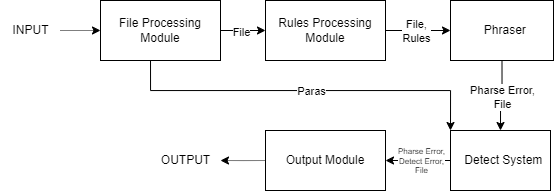
\includegraphics[width=3.3in]{figures/originprocess.png}
  \caption{Origin Process}
  \label{fig:originprocess}
  \end{figure}

  \begin{figure}[h]
    \centering
    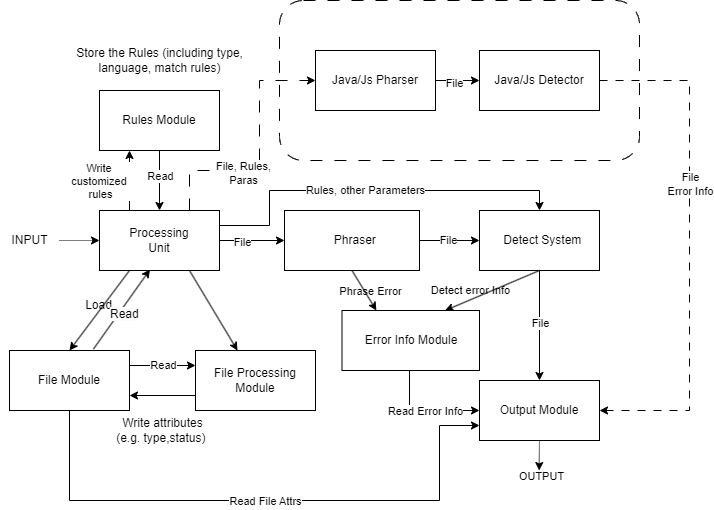
\includegraphics[width=3.3in]{figures/tdprocess.png}
    \caption{TD Process}
    \label{fig:tdprocess}
    \end{figure}

\subsubsection{Testing and Deployment}
In the final part of this sprint, we mainly continue to address the non-functional requirements of the software, such as its maintainability, runtime efficiency, thread-safety, and performance under stress testing.

First, we deployed the software on a server (see the Security Assessment chapter for server configuration details) to facilitate developer access, use, and testing, thus improving system maintainability. We only need to update the code locally and regularly deploy the new program to the server to form new versions, making maintenance work easier for developers. In addition, to assess the efficiency of the detection software, we evaluate whether the system can quickly respond to user needs and provide corresponding code detection from various perspectives, including runtime efficiency, transaction throughput, success rate, and response time. At the same time, we conducted load and stress tests on the system to assess its performance under high-data-volume and multi-threaded testing conditions. Since we had previously focused on unit tests, ensuring the performance of individual modules, we couldn't guarantee that situations such as deadlocks wouldn't occur under multi-threaded conditions or verify the software's efficiency during concurrent situations. Therefore, we verified the software's performance in these aspects through stress and load tests.

\section{Evaluation}
\noindent The Evaluation section summarizes the verification and evaluation processes applied to the solution. It outlines how the team gauged the effectiveness of the tool in solving the identified code smell problems. Special attention is given to scalability considerations, comparing the results to existing tools in the software engineering landscape.

\subsection{Security Evaluation}
The evaluation dives into the scalability of the developed tools, exploring their performance in handling varying codebase sizes. This section utilizes equations and figures to demonstrate scalability metrics. A comparative analysis with existing tools further validates the tool's efficacy.

\subsubsection{Session Management}
The session management functionality comes into play after a user successfully logs in. The user's identifier (i.e., user ID) is stored in the session, and the user's login status can be verified by checking the identifier in the session. This ensures that only authenticated users can access restricted features. For example, we can set that only the user with session ID 2 (i.e., the administrator) can view log records. Additionally, session management has other benefits, such as storing user identifiers in the session so that users can remain logged in even after closing the browser, without needing to log in again.

\subsubsection{User Input Validation and Sanitization}
The code includes input validation or sanitization to prevent security vulnerabilities such as SQL injection and cross-site scripting (XSS) attacks. We use the \verb|bleach.clean()| function to sanitize the username and password inputs provided by users. This function removes HTML tags from the input to prevent cross-site scripting (XSS) attacks. Additionally, we validate that the username and password are not empty and return appropriate error messages in case of errors.

\subsubsection{Database Queries}
We use parameterized queries to prevent SQL injection attacks. The variable parts of the database queries are represented using placeholders (e.g., \verb|`?`| or \verb|`%s`|) and the variable values are passed as parameters to the queries. This ensures that user inputs are properly escaped and handled, thereby preventing injection attacks.

\subsubsection{Password Storage}
The \verb|werkzeug.security| module was used for password hashing. Password hashing helps protect the security of user passwords, even if the database is compromised, as attackers cannot easily reverse engineer the passwords. This enhances the security of the application and protects users' sensitive information.

\subsubsection{Principle of Least Privilege}
In terms of database connectivity, we use a database user with appropriate privileges for the connection, avoiding the use of a user with excessive privileges. We grant the user with ID 2 the necessary permissions to access the log database, and they cannot perform unauthorized access to other sensitive data or operations. This practice helps enhance system security and protect sensitive information in the database.

\subsubsection{Security Framework}
We use the secure React framework for the frontend and the Flask framework for the backend. The security of the React framework is demonstrated through features such as the virtual DOM, component isolation, prop validation, and scaffolding tools. It manages page rendering and updates through the virtual DOM, encourages component-based development for data and functionality isolation, provides prop validation mechanisms, and offers scaffolding tools to assist developers in building secure applications.
The security of the Flask framework is manifested in functionalities such as route protection, authentication and authorization, form validation, and handling of security-related headers. It provides protection for sensitive routes and functionalities, supports various authentication and authorization mechanisms, can validate user-submitted data, and automatically handles security-related HTTP headers.

\subsection{Scalability Evaluation}
\label{evaluate:Scalability}

Scalability is a critical aspect of our code smell detection tool, as it determines its ability to handle diverse and large-scale software projects efficiently. The evaluation involves several key components:

\subsubsection{Test Scenarios}

We conducted scalability tests across a spectrum of software projects, ranging from small-scale applications to large enterprise-level systems. This diversity ensures that our tool's performance is assessed under realistic conditions.

\subsubsection{Metrics}

To quantify scalability, we measured the tool's performance based on key metrics, including execution time, memory usage, and response time. These metrics provide insights into how well the tool handles increasing codebase sizes without significant degradation in performance.

\subsubsection{Comparison with Existing Tools}

To contextualize our results, we compared the scalability of our tool with existing code smell detection tools in the industry. This comparative analysis offers a benchmark for understanding the tool's performance relative to established solutions.

\subsubsection{Scalability Equations}

We utilized scalability equations to model the tool's performance as the size of the codebase increases. These equations help predict how the tool will scale in different scenarios and provide valuable insights for future users.

\subsubsection{Parallel Processing}

Incorporating principles covered in software engineering, our tool utilizes parallel processing techniques to enhance scalability. This involves efficiently distributing the workload across multiple processing units, mitigating bottlenecks and improving overall performance.

\subsubsection{Dynamic Scaling}

Our tool employs dynamic scaling mechanisms, adjusting resource allocation based on the size and complexity of the codebase being analyzed. This adaptive approach ensures optimal performance across a wide range of scenarios.

\subsubsection{Results and Analysis}

The scalability evaluation yielded promising results, showcasing our tool's ability to efficiently handle diverse codebases. Execution times remained within acceptable limits even as project sizes increased. Memory usage demonstrated stability, and response times were consistently low.

Comparison with existing tools highlighted the competitive scalability of our solution, positioning it as a viable option for developers working on projects of varying scales.

\subsubsection{Future Considerations}

To ensure continued scalability as software projects evolve, we outline plans for future enhancements. This includes ongoing optimization efforts, monitoring for potential bottlenecks, and incorporating feedback from users to address specific scalability challenges in real-world scenarios.

\subsection{Performance Evaluation}

\subsubsection{Environment preparation}
Load testing environment:
CPU configuration: i5-12490F,
Operating system: Windows 11,
Memory size: 16GB,
Load testing tool: Locust,
Monitoring tool: Python code to monitor CPU utilization

Server environment1:
CPU configuration: Intel Xeon Platinum 8370C (1) @ 2.793GHz,
Operating system: Debian GNU\/Linux 11 (bullseye) x86\_64,
Kernel Version: 5.10.0-26-cloud-amd64,
Memory size: 914MiB

Server environment2:
CPU configuration: ARM Neoverse-N1 (2),
Operating system: Gentoo Linux aarch64,
Kernel Version: 6.1.57-gentoo-dist,
Memory size: 11945MiB

\begin{figure}[h]
  \centering
\subfloat[Server environment 1 - Limitation x86\_64 Server\label{fig:srv1}]{%
     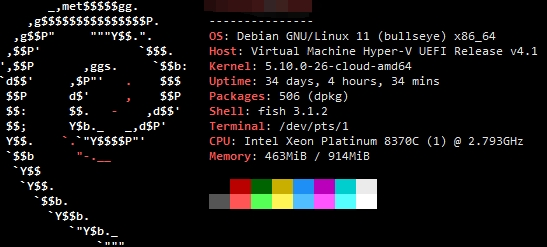
\includegraphics[width=1\linewidth]{figures/evalusrv1.png}}
  \hfill
\subfloat[Server environment 2 - Performance Arm64 Server\label{fig:srv2}]{%
      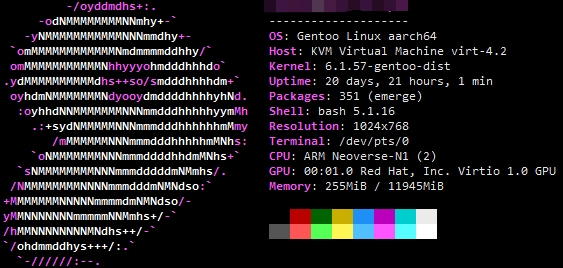
\includegraphics[width=1\linewidth]{figures/evalusrv2.png}}
\caption{Server environment}
\label{fig:evalusrv} 
\end{figure}


\subsubsection{Locust}
Locust is a load testing tool that is described using pure Python scripts and is based entirely on the Requests library for making HTTP requests. The Requests library is simple and easy to use, yet powerful in functionality.

Unlike other load testing tools, Locust utilizes the concurrency mechanism of coroutines (gevent) instead of using processes and threads. When using multiple threads to simulate multiple users, the number of threads increases with the concurrency level. However, thread switching consumes resources, and IO blocking and thread sleep inevitably reduce concurrency efficiency. Therefore, testing tools like LoadRunner and JMeter, which use processes and threads, struggle to simulate high concurrency pressure on a single machine.

In contrast, Locust's coroutine mechanism avoids system-level resource scheduling, significantly improving performance. This means that on an ordinary configuration test machine, it is effortless to generate thousands of concurrent requests.


\subsubsection{Performance metrics} We use different metrics for the evaluation.

\textbf{Business performance metrics}
\begin{itemize}
  \item Concurrency level: The concurrency level refers to the number of users who are simultaneously sending requests and interacting with the system. It reflects the system's ability to handle concurrent requests.
  \item Transaction Throughput (TPS/RPS): Transaction throughput refers to the number of transactions or requests that a system can process within a unit of time. It represents the system's processing capacity and performance.
  \item Average Transaction Response Time: The average transaction response time refers to the average time it takes for the system to process a transaction. It measures the system's responsiveness to user requests.
  \item Transaction Success Rate: The transaction success rate is the ratio of successfully processed transactions to the total number of transactions. It reflects the system's stability and reliability.
\end{itemize}

\textbf{System resource performance metrics}
\begin{itemize}
  \item CPU utilization: CPU utilization indicates the extent to which the CPU is being used in the system, i.e., the workload on the CPU within a unit of time. It can measure the system's computing capacity and its ability to handle the load.
  \item Memory utilization: Memory utilization refers to the ratio between the used memory and the total memory in the system. It reflects the system's occupation of memory resources, and high memory utilization can potentially lead to decreased system performance or memory overflow.
\end{itemize}


\subsubsection{Performance testing}
Test code (partial)
\begin{lstlisting}[caption={Test code (partial)},label={lst:testcode},language=python,breaklines=true]
class UserBehavior(HttpUser):
    wait_time = between(1, 5)
    host = "http://127.0.0.1:5000"
    cpu_data = []
    memory_data = []
    @task
    def login(self):
        cpu_percent = psutil.cpu_percent()
        memory_percent = psutil.virtual_memory().percent
        self.cpu_data.append(cpu_percent)
        self.memory_data.append(memory_percent)
        response = self.client.get('/login')

    @task
    def do_login_and_out(self):
        cpu_percent = psutil.cpu_percent()
        memory_percent = psutil.virtual_memory().percent
        self.cpu_data.append(cpu_percent)
        self.memory_data.append(memory_percent)
        headers = {'Content-Type': 'application/x-www-form-urlencoded'}
        data = {
            'username': '123',
            'password': '123'
        }
        response = self.client.post('/dologin', headers=headers, data=data)
        response = self.client.get('/logout')
  \end{lstlisting}

\textbf{Standard Testing} aims to determine the performance level of a system under normal conditions. For this project, we will simulate 10 users executing the test code within 1 minute. 
\begin{lstlisting}[label={lst:locustcmd1},language=BASH,breaklines=true]
locust -f your_test_file.py --headless -u 10 -r 1 --run-time 1m
\end{lstlisting}

\textbf{Execution results:}

Request statistics results shown in Table \ref{tab:stdreqstat} and Fig.\ref{fig:stdreqstat}.

\begin{table*}[h]
  \caption{Standard Testing Request Statistics}
  \label{tab:stdreqstat}
  \begin{tabular}{|l|l|l|l|l|l|l|l|l|l|}
  \hline
  \multicolumn{1}{|c|}{\textbf{Method}} & \multicolumn{1}{c|}{\textbf{Name}} & \multicolumn{1}{c|}{\textbf{\# Requests}} & \multicolumn{1}{c|}{\textbf{\# Fails}} & \multicolumn{1}{c|}{\textbf{Average (ms)}} & \multicolumn{1}{c|}{\textbf{Min (ms)}} & \multicolumn{1}{c|}{\textbf{Max (ms)}} & \multicolumn{1}{c|}{\textbf{Average size (bytes)}} & \multicolumn{1}{c|}{\textbf{RPS}} & \multicolumn{1}{c|}{\textbf{Failures/s}} \\ \hline
  GET                                   & /dashboard                         & 23                                        & 0                                      & 6                                          & 3                                      & 31                                     & 528                                                & 0.4                               & 0.0                                      \\ \hline
  {\color[HTML]{2A2B2E} POST}           & /dologin                           & 30                                        & 0                                      & 98                                         & 90                                     & 122                                    & 5472                                               & 0.5                               & 0.0                                      \\ \hline
  {\color[HTML]{2A2B2E} POST}           & /doupload                          & 32                                        & 0                                      & 2                                          & 1                                      & 16                                     & 45                                                 & 0.5                               & 0.0                                      \\ \hline
  POST                                  & /dourlfetch                        & 28                                        & 0                                      & 2                                          & 1                                      & 6                                      & 39                                                 & 0.5                               & 0.0                                      \\ \hline
  POST                                  & /dovuldetect                       & 29                                        & 0                                      & 1                                          & 1                                      & 2                                      & 39                                                 & 0.5                               & 0.0                                      \\ \hline
  POST                                  & /dovulfetch                        & 28                                        & 0                                      & 2                                          & 1                                      & 3                                      & 39                                                 & 0.5                               & 0.0                                      \\ \hline
  GET                                   & /login                             & 21                                        & 0                                      & 2                                          & 1                                      & 3                                      & 528                                                & 0.4                               & 0.0                                      \\ \hline
  GET                                   & /logout                            & 30                                        & 0                                      & 3                                          & 2                                      & 3                                      & 528                                                & 0.5                               & 0.0                                      \\ \hline
                                        & Aggregated                         & 221                                       & 0                                      & 15                                         & 1                                      & 122                                    & 941                                                & 3.7                               & 0.0                                      \\ \hline
  \end{tabular}
  \end{table*}
% Please add the following required packages to your document preamble:
% \usepackage[table,xcdraw]{xcolor}
% Beamer presentation requires \usepackage{colortbl} instead of \usepackage[table,xcdraw]{xcolor}
\begin{table*}[]
  \caption{Standard Testing Response Time Statistics}
  \label{tab:stdrespstat}
  \begin{tabular}{|l|l|l|l|l|l|l|l|l|l|}
  \hline
  \multicolumn{1}{|c|}{\textbf{Method}} & \multicolumn{1}{c|}{\textbf{Name}} & \multicolumn{1}{c|}{\textbf{50\%ile (ms)}} & \multicolumn{1}{c|}{\textbf{60\%ile (ms)}} & \multicolumn{1}{c|}{\textbf{70\%ile (ms)}} & \multicolumn{1}{c|}{\textbf{80\%ile (ms)}} & \multicolumn{1}{c|}{\textbf{90\%ile (ms)}} & \multicolumn{1}{c|}{\textbf{95\%ile (ms)}} & \multicolumn{1}{c|}{\textbf{99\%ile (ms)}} & \multicolumn{1}{c|}{\textbf{100\%ile (ms)}} \\ \hline
  GET                                   & /dashboard                         & 3                                          & 3                                          & 4                                          & 5                                          & 9                                          & 30                                         & 31                                         & 31                                          \\ \hline
  {\color[HTML]{2A2B2E} POST}           & /dologin                           & 93                                         & 95                                         & 100                                        & 110                                        & 120                                        & 120                                        & 120                                        & 120                                         \\ \hline
  {\color[HTML]{2A2B2E} POST}           & /doupload                          & 2                                          & 2                                          & 2                                          & 3                                          & 3                                          & 4                                          & 16                                         & 16                                          \\ \hline
  POST                                  & /dourlfetch                        & 2                                          & 2                                          & 2                                          & 2                                          & 3                                          & 3                                          & 6                                          & 6                                           \\ \hline
  POST                                  & /dovuldetect                       & 2                                          & 2                                          & 2                                          & 2                                          & 2                                          & 2                                          & 2                                          & 2                                           \\ \hline
  POST                                  & /dovulfetch                        & 2                                          & 2                                          & 2                                          & 2                                          & 3                                          & 3                                          & 3                                          & 3                                           \\ \hline
  GET                                   & /login                             & 2                                          & 2                                          & 2                                          & 2                                          & 3                                          & 3                                          & 3                                          & 3                                           \\ \hline
  GET                                   & /logout                            & 3                                          & 3                                          & 3                                          & 3                                          & 3                                          & 4                                          & 4                                          & 4                                           \\ \hline
                                        & Aggregated                         & 2                                          & 3                                          & 3                                          & 3                                          & 92                                         & 95                                         & 120                                        & 120                                         \\ \hline
  \end{tabular}
  \end{table*}
\begin{table*}[h]
  \caption{Load Testing Request Statistics}
  \label{tab:loadreqstat}
  \begin{tabular}{|p{0.07\textwidth}|p{0.1\textwidth}|p{0.07\textwidth}|p{0.07\textwidth}|p{0.07\textwidth}|p{0.07\textwidth}|p{0.07\textwidth}|p{0.07\textwidth}|p{0.07\textwidth}|p{0.07\textwidth}|}
    \hline
    {\textbf{Method}} & {\textbf{Name}} & {\textbf{\# Requests}} & {\textbf{\# Fails}} & {\textbf{Average (ms)}} & {\textbf{Min (ms)}} & {\textbf{Max (ms)}} & {\textbf{Average size (bytes)}} & {\textbf{RPS}} & {\textbf{Failures/s}} \\ \hline
    GET                                   & /dashboard                         & 1424                                      & 0                                      & 4                                          & 2                                      & 25                                     & 528                                                & 2.4                               & 0.0                                      \\ \hline
    {\color[HTML]{2A2B2E} POST}           & /dologin                           & 1429                                      & 11                                     & 111                                        & 90                                     & 221                                    & 5431                                               & 2.4                               & 0.0                                      \\ \hline
    {\color[HTML]{2A2B2E} POST}           & /doupload                          & 1433                                      & 0                                      & 2                                          & 1                                      & 22                                     & 45                                                 & 2.4                               & 0.0                                      \\ \hline
    POST                                  & /dourlfetch                        & 1374                                      & 2                                      & 2                                          & 1                                      & 42                                     & 38                                                 & 2.3                               & 0.0                                      \\ \hline
    POST                                  & /dovuldetect                       & 1399                                      & 0                                      & 2                                          & 1                                      & 23                                     & 39                                                 & 2.3                               & 0.0                                      \\ \hline
    POST                                  & /dovulfetch                        & 1416                                      & 0                                      & 2                                          & 1                                      & 16                                     & 39                                                 & 2.4                               & 0.0                                      \\ \hline
    GET                                   & /login                             & 1470                                      & 0                                      & 2                                          & 1                                      & 42                                     & 528                                                & 2.5                               & 0.0                                      \\ \hline
    GET                                   & /logout                            & 1429                                      & 0                                      & 3                                          & 2                                      & 27                                     & 528                                                & 2.4                               & 0.0                                      \\ \hline
                                          & Aggregated                         & 11374                                     & 13                                     & 16                                         & 1                                      & 221                                    & 903                                                & 19.0                              & 0.0                                      \\ \hline
    \end{tabular}
  \end{table*}
% Please add the following required packages to your document preamble:
% \usepackage[table,xcdraw]{xcolor}
% Beamer presentation requires \usepackage{colortbl} instead of \usepackage[table,xcdraw]{xcolor}
\begin{table*}[]
  \caption{Load Testing Response Time Statistics}
  \label{tab:loadrespstat}
  \begin{tabular}{|p{0.07\textwidth}|p{0.1\textwidth}|p{0.07\textwidth}|p{0.07\textwidth}|p{0.07\textwidth}|p{0.07\textwidth}|p{0.07\textwidth}|p{0.07\textwidth}|p{0.07\textwidth}|p{0.07\textwidth}|}
    \hline
{\textbf{Method}} & {\textbf{Name}} & {\textbf{50\%ile (ms)}} & {\textbf{60\%ile (ms)}} & {\textbf{70\%ile (ms)}} & {\textbf{80\%ile (ms)}} & {\textbf{90\%ile (ms)}} & {\textbf{95\%ile (ms)}} & {\textbf{99\%ile (ms)}} & {\textbf{100\%ile (ms)}} \\ \hline
GET                                   & /dashboard                         & 4                                          & 4                                          & 5                                          & 5                                          & 6                                          & 7                                          & 10                                         & 26                                          \\ \hline
{\color[HTML]{2A2B2E} POST}           & /dologin                           & 100                                        & 110                                        & 110                                        & 120                                        & 140                                        & 150                                        & 180                                        & 220                                         \\ \hline
{\color[HTML]{2A2B2E} POST}           & /doupload                          & 2                                          & 2                                          & 3                                          & 3                                          & 4                                          & 5                                          & 12                                         & 22                                          \\ \hline
POST                                  & /dourlfetch                        & 2                                          & 2                                          & 3                                          & 3                                          & 4                                          & 5                                          & 8                                          & 42                                          \\ \hline
POST                                  & /dovuldetect                       & 2                                          & 2                                          & 3                                          & 3                                          & 4                                          & 5                                          & 8                                          & 23                                          \\ \hline
POST                                  & /dovulfetch                        & 2                                          & 2                                          & 3                                          & 3                                          & 4                                          & 5                                          & 7                                          & 16                                          \\ \hline
GET                                   & /login                             & 2                                          & 2                                          & 3                                          & 3                                          & 4                                          & 5                                          & 8                                          & 42                                          \\ \hline
GET                                   & /logout                            & 3                                          & 3                                          & 3                                          & 4                                          & 4                                          & 5                                          & 7                                          & 27                                          \\ \hline
                                      & Aggregated                         & 3                                          & 3                                          & 4                                          & 5                                          & 97                                         & 110                                        & 150                                        & 220                                         \\ \hline
\end{tabular}
  \end{table*}
\begin{table*}[h]
  \caption{Fatigue Strength Testing Request Statistics}
  \label{tab:fstreqstat}
  \begin{tabular}{|l|l|l|l|l|l|l|l|l|l|}
    \hline
    \multicolumn{1}{|c|}{\textbf{Method}} & \multicolumn{1}{c|}{\textbf{Name}} & \multicolumn{1}{c|}{\textbf{\# Requests}} & \multicolumn{1}{c|}{\textbf{\# Fails}} & \multicolumn{1}{c|}{\textbf{Average (ms)}} & \multicolumn{1}{c|}{\textbf{Min (ms)}} & \multicolumn{1}{c|}{\textbf{Max (ms)}} & \multicolumn{1}{c|}{\textbf{Average size (bytes)}} & \multicolumn{1}{c|}{\textbf{RPS}} & \multicolumn{1}{c|}{\textbf{Failures/s}} \\ \hline
    GET                                   & /dashboard                         & 5102                                      & 0                                      & 4                                          & 2                                      & 32                                     & 528                                                & 1.4                               & 0.0                                      \\ \hline
    POST                                  & /dologin                           & 5099                                      & 7                                      & 105                                        & 88                                     & 230                                    & 5464                                               & 1.4                               & 0.0                                      \\ \hline
    POST                                  & /doupload                          & 5043                                      & 4                                      & 2                                          & 1                                      & 16                                     & 44                                                 & 1.4                               & 0.0                                      \\ \hline
    POST                                  & /dourlfetch                        & 5136                                      & 7                                      & 2                                          & 1                                      & 37                                     & 38                                                 & 1.4                               & 0.0                                      \\ \hline
    POST                                  & /dovuldetect                       & 5143                                      & 6                                      & 2                                          & 1                                      & 19                                     & 38                                                 & 1.4                               & 0.0                                      \\ \hline
    POST                                  & /dovulfetch                        & 5098                                      & 0                                      & 2                                          & 1                                      & 27                                     & 39                                                 & 1.4                               & 0.0                                      \\ \hline
    GET                                   & /login                             & 5078                                      & 0                                      & 2                                          & 1                                      & 33                                     & 528                                                & 1.4                               & 0.0                                      \\ \hline
    GET                                   & /logout                            & 5099                                      & 0                                      & 3                                          & 2                                      & 32                                     & 528                                                & 1.4                               & 0.0                                      \\ \hline
                                          & Aggregated                         & 40798                                     & 24                                     & 15                                         & 1                                      & 230                                    & 900                                                & 11.3                              & 0.0                                      \\ \hline
    \end{tabular}
  \end{table*}
% Please add the following required packages to your document preamble:
% \usepackage[table,xcdraw]{xcolor}
% Beamer presentation requires \usepackage{colortbl} instead of \usepackage[table,xcdraw]{xcolor}
\begin{table*}[]
  \caption{Fatigue Strength Testing Response Time Statistics}
  \label{tab:fstrespstat}
  \begin{tabular}{|l|l|l|l|l|l|l|l|l|l|}
    \hline
    \multicolumn{1}{|c|}{\textbf{Method}} & \multicolumn{1}{c|}{\textbf{Name}} & \multicolumn{1}{c|}{\textbf{50\%ile (ms)}} & \multicolumn{1}{c|}{\textbf{60\%ile (ms)}} & \multicolumn{1}{c|}{\textbf{70\%ile (ms)}} & \multicolumn{1}{c|}{\textbf{80\%ile (ms)}} & \multicolumn{1}{c|}{\textbf{90\%ile (ms)}} & \multicolumn{1}{c|}{\textbf{95\%ile (ms)}} & \multicolumn{1}{c|}{\textbf{99\%ile (ms)}} & \multicolumn{1}{c|}{\textbf{100\%ile (ms)}} \\ \hline
    GET                                   & /dashboard                         & 3                                          & 4                                          & 4                                          & 4                                          & 5                                          & 6                                          & 17                                         & 33                                          \\ \hline
    POST                                  & /dologin                           & 97                                         & 100                                        & 110                                        & 120                                        & 130                                        & 140                                        & 160                                        & 230                                         \\ \hline
    POST                                  & /doupload                          & 2                                          & 2                                          & 2                                          & 3                                          & 3                                          & 4                                          & 6                                          & 17                                          \\ \hline
    POST                                  & /dourlfetch                        & 2                                          & 2                                          & 2                                          & 3                                          & 3                                          & 4                                          & 15                                         & 38                                          \\ \hline
    POST                                  & /dovuldetect                       & 2                                          & 2                                          & 2                                          & 3                                          & 4                                          & 4                                          & 13                                         & 20                                          \\ \hline
    POST                                  & /dovulfetch                        & 2                                          & 2                                          & 2                                          & 3                                          & 3                                          & 4                                          & 6                                          & 27                                          \\ \hline
    GET                                   & /login                             & 2                                          & 2                                          & 2                                          & 3                                          & 3                                          & 4                                          & 14                                         & 33                                          \\ \hline
    GET                                   & /logout                            & 3                                          & 3                                          & 3                                          & 4                                          & 4                                          & 5                                          & 15                                         & 32                                          \\ \hline
                                          & Aggregated                         & 3                                          & 3                                          & 3                                          & 4                                          & 92                                         & 100                                        & 130                                        & 230                                         \\ \hline
    \end{tabular}
  \end{table*}

  \begin{figure*}[!t]
    \centering
  \subfloat[Standard Testing\label{a}]{%
       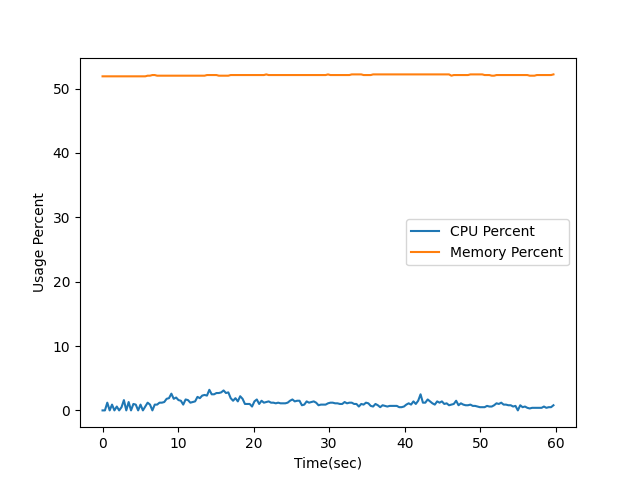
\includegraphics[width=0.24\textwidth]{figures/srvstat1.png}}
    \hfill
  \subfloat[Load Testing\label{b}]{%
        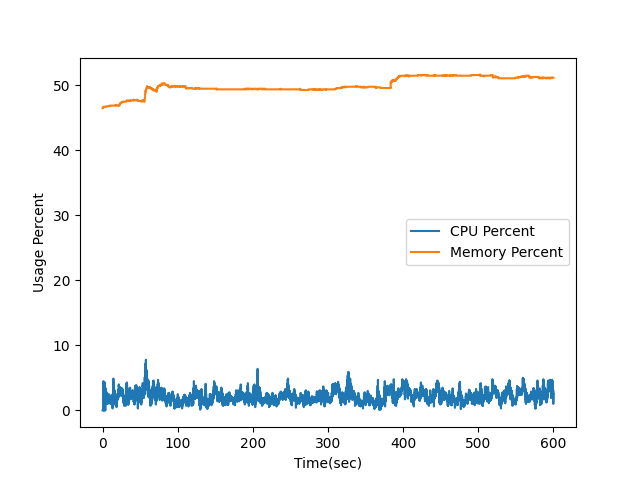
\includegraphics[width=0.24\textwidth]{figures/srvstat2.png}}
    \hfill
  \subfloat[Stress testing\label{c}]{%
        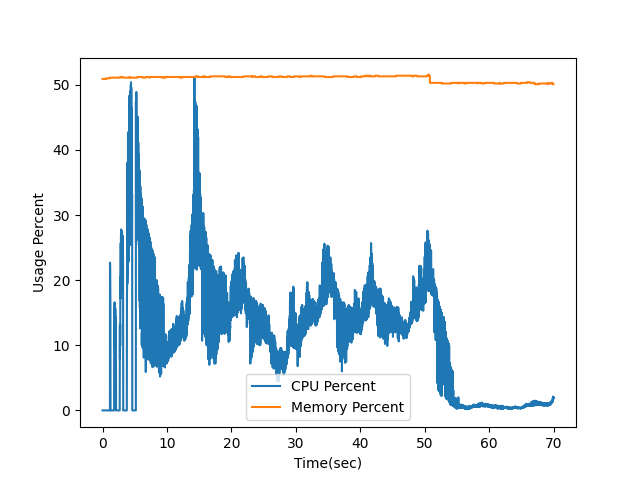
\includegraphics[width=0.24\textwidth]{figures/srvstat3.png}}
    \hfill
  \subfloat[Fatigue Strength Testing\label{d}]{%
        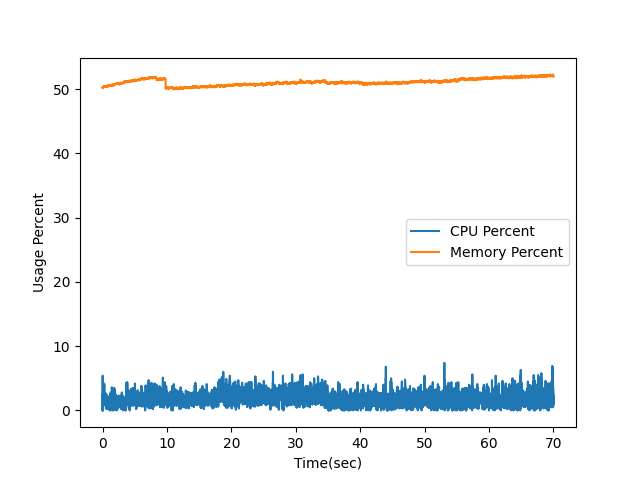
\includegraphics[width=0.24\textwidth]{figures/srvstat4.png}}
  \caption{Server Status via Testing.}
  \label{fig:srvstats} 
\end{figure*}

\begin{figure}[h]
  \centering
  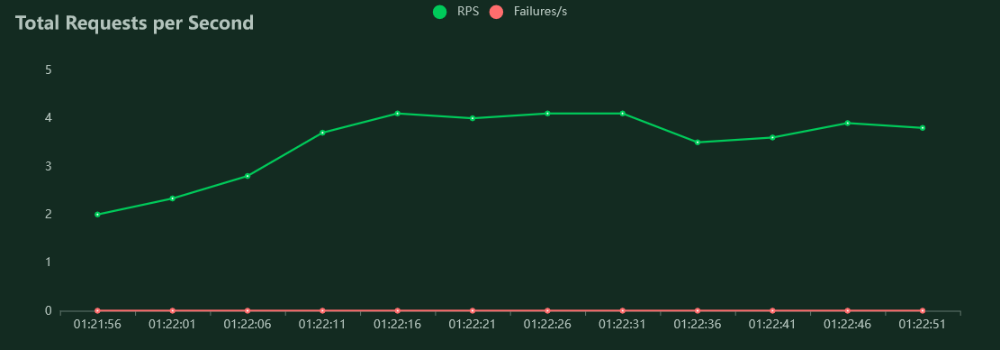
\includegraphics[width=3.4in]{figures/stdreqstat.png}
  \caption{Standard Testing Request statistics}
  \label{fig:stdreqstat}
  \end{figure}


Response Time Statistics results shown in Table \ref{tab:stdrespstat} and Fig.\ref{fig:stdrespstat}

\begin{figure}[h]
  \centering
  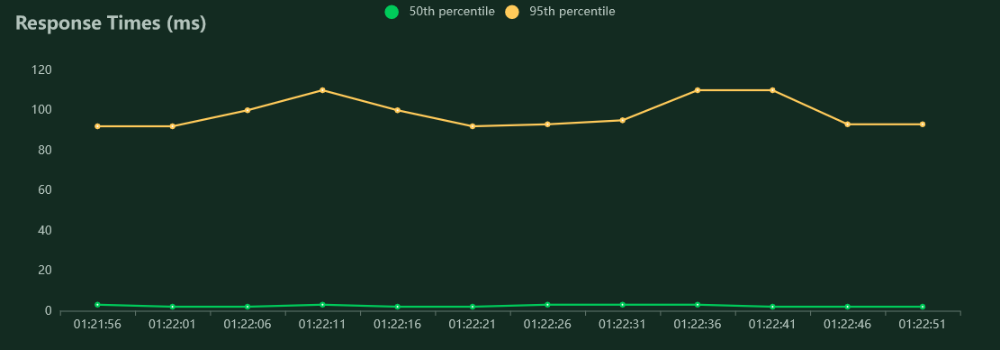
\includegraphics[width=3.4in]{figures/stdrespstat.png}
  \caption{Standard Testing Request statistics}
  \label{fig:stdrespstat}
  \end{figure}

\textbf{Load Testing} aims to evaluate the performance and stability of a system under normal and peak loads. It involves simulating a certain number of concurrent users performing tasks. For this experiment, we will simulate 50 concurrent users executing tasks at a rate of 10 requests per second for a duration of 10 minutes. 
\begin{lstlisting}[label={lst:locustcmd2},language=BASH,breaklines=true]
locust -f your_test_file.py --headless -u 50 -r 10 --run-time 10m 
\end{lstlisting}

Request statistics results shown in Table \ref{tab:loadreqstat} and Fig.\ref{fig:loadreqstat}.

\begin{figure}[h]
  \centering
  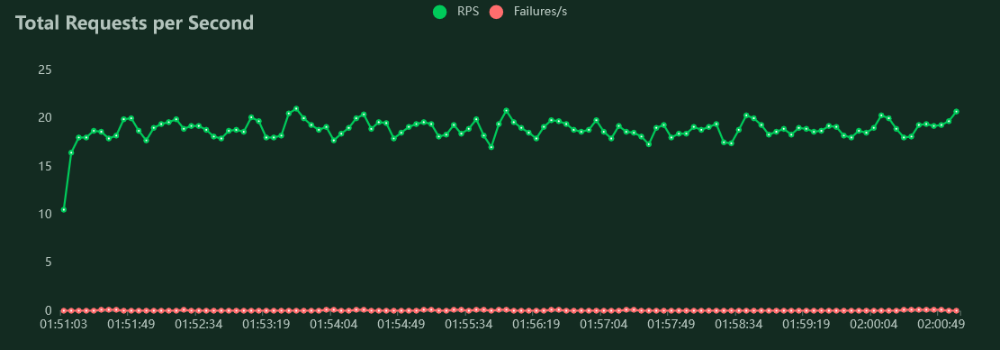
\includegraphics[width=3.4in]{figures/loadreqstat.png}
  \caption{Load Testing Request statistics}
  \label{fig:loadreqstat}
  \end{figure}



Response Time Statistics results shown in Table \ref{tab:loadrespstat} and Fig.\ref{fig:loadrespstat}, The Failures Statistics shown in Table \ref{tab:failureseva}.


\begin{figure}[h]
  \centering
  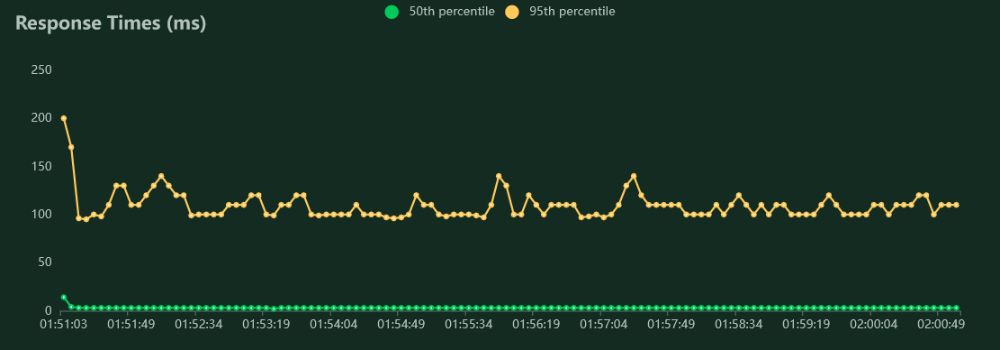
\includegraphics[width=3.4in]{figures/loadrespstat.png}
  \caption{Load Testing Request statistics}
  \label{fig:loadrespstat}
  \end{figure}

\textbf{Stress testing} aims to evaluate the performance and resilience of a system under overload conditions. It involves increasing the testing load by either increasing the number of concurrent users or the frequency of task execution to simulate higher levels of stress. For this experiment, we will simulate 300 concurrent users executing tasks at a rate of 50 requests per second for a duration of 30 minutes.
\begin{lstlisting}[label={lst:locustcmd3},language=BASH,breaklines=true]
locust -f your_test_file.py --headless -u 300 -r 50 --run-time 30m 
\end{lstlisting}

From the analysis of the Fig.\ref{fig:stressreqstat} and Fig.\ref{fig:stressrespstat}, it can be observed that the system experienced a crash during the operation under high load conditions.

\begin{figure}[h]
  \centering
  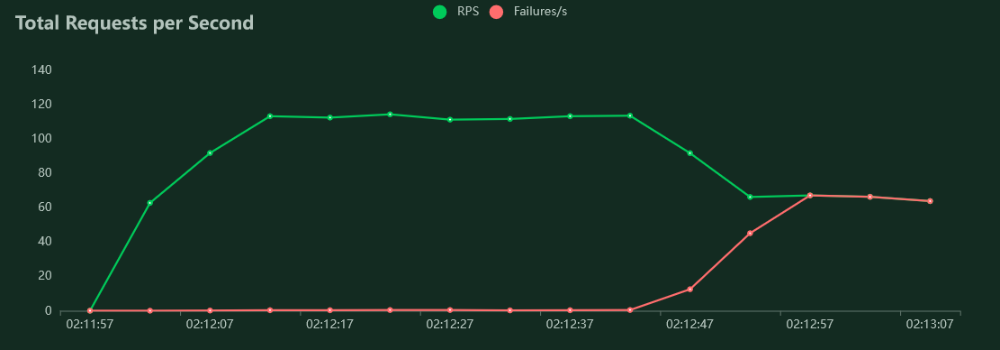
\includegraphics[width=3.4in]{figures/stressreqstat.png}
  \caption{Stress Testing Request statistics}
  \label{fig:stressreqstat}
  \end{figure}

\begin{figure}[h]
  \centering
  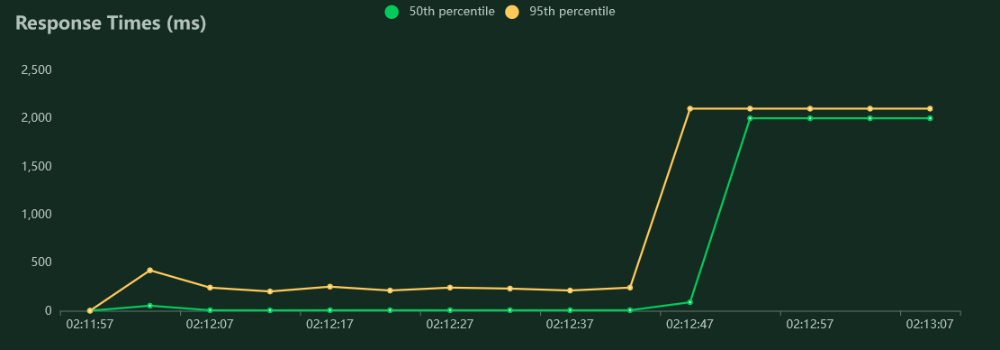
\includegraphics[width=3.4in]{figures/stressrespstat.png}
  \caption{Stress Testing Request statistics}
  \label{fig:stressrespstat}
  \end{figure}

\textbf{Fatigue Strength Testing} aims to evaluate the stability and reliability of a system under sustained load conditions. It involves running tests for an extended period of time and observing the system's performance and resource utilization during prolonged operation. For this experiment, we will simulate 30 concurrent users executing tasks at a rate of 5 requests per second for a duration of 1 hour. 
\begin{lstlisting}[label={lst:locustcmd4},language=BASH,breaklines=true]
locust -f your_test_file.py --headless -u 30 -r 5 --run-time 1h 
\end{lstlisting}

Request statistics results shown in Table \ref{tab:fstreqstat} and Fig.\ref{fig:fstreqstat}.

\begin{figure}[h]
  \centering
  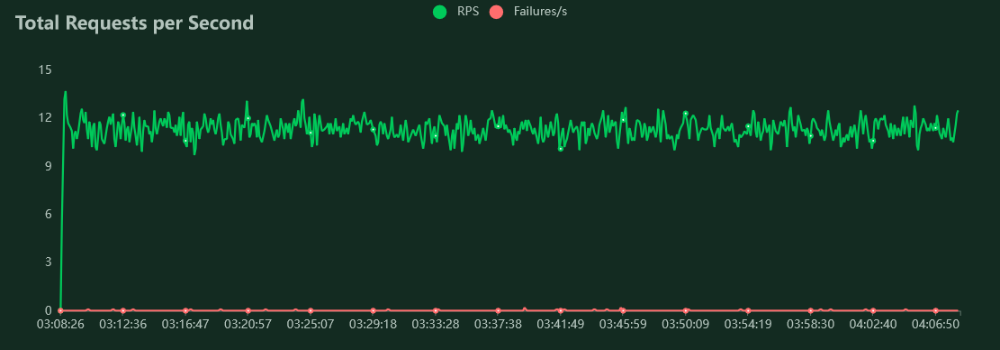
\includegraphics[width=3.4in]{figures/fstreqstat.png}
  \caption{Fatigue Strength Testing Request statistics}
  \label{fig:fstreqstat}
  \end{figure}
\begin{figure}[h]
  \centering
  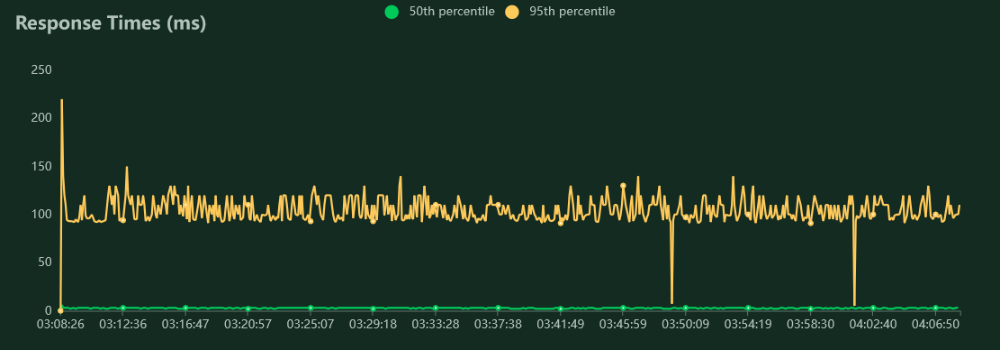
\includegraphics[width=3.4in]{figures/fstrespstat.png}
  \caption{Fatigue Strength Testing Request statistics}
  \label{fig:fstrespstat}
  \end{figure}

Response Time Statistics results shown in Table \ref{tab:fstrespstat} and Fig.\ref{fig:fstrespstat}.

\begin{table}[h]
\caption{Failures Statistics}
\label{tab:failureseva}
\begin{tabular}{|p{0.1\linewidth}|p{0.15\linewidth}|p{0.25\linewidth}|p{0.1\linewidth}|}
\hline
\multicolumn{1}{|c|}{\textbf{Method}} & \multicolumn{1}{c|}{\textbf{Name}} & \multicolumn{1}{c|}{\textbf{Error}}                       & \multicolumn{1}{c|}{\textbf{Occurrences}} \\ \hline
POST                                  & /dologin                           & 500 Server Error: INTERNAL SERVER ERROR for url: /dologin & 11                                        \\ \hline
POST                                  & /dourlfetch                        & {[}WinError 10053{]}                 & 2                                         \\ \hline
\end{tabular}
\end{table}

\section{Conclusion and Future Work}
\noindent In conclusion, we delivered a functional multi-language security scanner successfully. This paper presented our project's development background, motivation, as well as some related work of recent research in the safety detection area. To make our solution clear, in the preliminaries part, we introduced the key technical method or framework used by our project. We also detailed the process, activities, techniques, deliverables, and outcomes involved in developing a web application security and code auditing tool over three sprints. In addition, we evaluated our system in a variety of testing. Summaries of each key part are as follows.

The introduction part highlighted rising cyber threats exploiting vulnerabilities in insecure code, emphasizing how most hacking incidents relate to flaws in system code. Manual code auditing was contrasted with automated methods that enable continuous, scalable, and bias-free assessments. Our tool aims to identify security weaknesses in apps as well as code written in Java, JavaScript, and PHP. It would assist developers in proactively strengthening application security and preventing exploits.

The related work reviewed prior papers in relevant domains like web security scanners, static analysis systems, machine learning approaches, and hybrid vulnerability detection tools.

The preliminaries provided background on common web vulnerabilities like SQL injection, XSS, SSRF, remote code execution, and URL redirection, explaining attack mechanisms. We also explain some technical concepts like front-end/back-end separation, React, Flask, CORS, Docker, and Kubernetes to readers.

The solution outlined the high-level design and modular architecture of the automated scanner. Key optimizations for modularity, extensibility, and reduced coupling were highlighted, including subclassing phrasers/detectors per language, generically handling intermediary logic, and encapsulating rule definitions. The section also covered solutions for enabling communication between the React front-end and Flask back-end across domains, using CORS headers and Nginx reverse proxy techniques. What's more, more details on team collaboration were mentioned, such as git branching strategy and collective code reviews.

The evaluation examined attributes like security, scalability, and performance. Security assessments include input validation, password encryption, and other techniques to prevent attacks. Scalability modeling tracks metrics like execution times and memory usage across diverse codebases. Load tests using Locust analyzed throughput, response times, and resource consumption under varied workloads.

As for our three sprints, the first sprint focused on defining the project scope and objectives, selecting appropriate programming frameworks, and designing the user interface. Through stakeholder interviews and prioritized into functional and non-functional categories, we gathered the requirements. Key requirements included SQL injection detection, common port scanning, DNS spoofing checks, and vulnerability detection for PHP, Java, and JavaScript code. Additionally, security and maintainability were identified as key non-functional requirements. Our team selected React, Flask, and custom algorithms as the frameworks for the front-end, back-end, and algorithms respectively. Interfaces were designed in this sprint. 

Sprint two centered on completing the development, followed by integration, deployment, and connectivity. The algorithm module delivered key website and code scanning features, though some vulnerability types were left out due to time constraints. The back-end provided business logic and database functionality but lacked performance for high-traffic loads. The front-end met requirements for website and code scanning pages as well as navigation and visual appeal, but couldn't deliver an in-page code editor. Integration tasks like exposing backend APIs and establishing front-end/back-end connectivity were completed successfully. 

The third sprint focused on documentation, security considerations, performance/scalability optimizations, resolving technical debt, and final testing/deployment. Documentation of requirements and interfaces was compiled and updated. Password encryption and input filtering addressed security concerns. Refactoring established inheritance relationships between language-specific and abstract base classes, enhancing extensibility. Previous quick additions of Java and JavaScript detection were integrated properly into the codebase. Stress testing, maintainability testing, and final deployment were also performed. 

In summary, our software engineering process resulted in a robust modular code auditing system offering website and source code scanning capabilities, which can detect several important application security vulnerabilities and weaknesses for key programming languages. Underlying design choices also make our system adaptable and scalable.  

\subsection*{Future Outlook}
After our reflection, we believe that there is still much room for improvement in our project. In future work, we can extend our detection language like C/C++, and Python, which would broaden vulnerability detection capabilities. For the web scanner, adding checks for other common threats like CORS misconfigurations would bolster security analysis. As a more powerful assistant for developers, the scanner should be coupled with auto-remediation modules to automatically fix discovered code flaws. From the related work, we also found machine learning approaches can potentially identify new classes of vulnerabilities and reduce false positives, which could be a new improvement direction for our project.



\bibliographystyle{ieeetr} 
\bibliography{refs} % Entries are in the refs.bib file

\vspace{-5 mm}
\begin{IEEEbiography}[{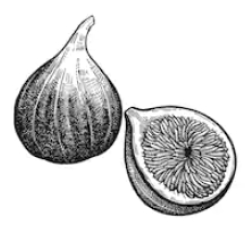
\includegraphics[width=1in,height=1.25in,clip,keepaspectratio]{figures/fig1.png}}]{Biography} According to the requirements that in the Project PPT. Biography is required. Such AS:\\
1. The bio of each student including the declaration of the contribution of the student.\\
2. Present a bio of each student. Who you are, your background, technical ideas, current interests, etc. Give a \textcolor{BurntOrange}{self-reflection} on the work done by you. \textcolor{BurntOrange}{State and justify your contribution} to the project.


\end{IEEEbiography}

\input{private/bio}

\end{document}


